\documentclass[12pt,oneside]{uhthesis}
\usepackage{subfigure}
\usepackage[ruled,lined,linesnumbered,titlenumbered,algochapter,spanish,onelanguage]{algorithm2e}
\usepackage{amsmath}
\usepackage{amssymb}
\usepackage{amsbsy}
\usepackage{caption,booktabs}
\captionsetup{ justification = centering }
%\usepackage{mathpazo}
\usepackage{float}			
\setlength{\marginparwidth}{2cm}
\usepackage{todonotes}
\usepackage{listings}
\usepackage{xcolor}
\usepackage{multicol}
\usepackage{graphicx}
\usepackage{subfigure}
\floatstyle{plaintop}
\restylefloat{table}
\addbibresource{Bibliography.bib}
% \setlength{\parskip}{\baselineskip}%
\renewcommand{\tablename}{Tabla}
\renewcommand{\listalgorithmcfname}{Índice de Algoritmos}
%\dontprintsemicolon
\SetAlgoNoEnd

\definecolor{codegreen}{rgb}{0,0.6,0}
\definecolor{codegray}{rgb}{0.5,0.5,0.5}
\definecolor{codepurple}{rgb}{0.58,0,0.82}
\definecolor{backcolour}{rgb}{0.95,0.95,0.92}

\lstdefinestyle{mystyle}{
    backgroundcolor=\color{backcolour},   
    commentstyle=\color{codegreen},
    keywordstyle=\color{purple},
    numberstyle=\tiny\color{codegray},
    stringstyle=\color{codepurple},
    basicstyle=\ttfamily\footnotesize,
    breakatwhitespace=false,         
    breaklines=true,                 
    captionpos=b,                    
    keepspaces=true,                 
    numbers=left,                    
    numbersep=5pt,                  
    showspaces=false,                
    showstringspaces=false,
    showtabs=false,                  
    tabsize=4
}

\lstset{style=mystyle}

\title{M\'odulo de modelos no lineales para el procesamiento de im\'agenes}
\author{\\\vspace{0.25cm}Carlos Toledo Silva}
\advisor{\\\vspace{0.25cm}Ms.C Dami\'an Vald\'es Santiago}
\degree{Licenciado en Ciencia de la Computación}
\faculty{Facultad de Matemática y Computación}
\date{25 de noviembre de 2022\\\vspace{0.25cm}\href{https://github.com/CTS-crypto/Logaritmic-Image-Processing}{https://github.com/CTS-crypto/Logaritmic-Image-Processing}}
\logo{Graphics/uhlogo}
\makenomenclature

\renewcommand{\vec}[1]{\boldsymbol{#1}}
\newcommand{\diff}[1]{\ensuremath{\mathrm{d}#1}}
\newcommand{\me}[1]{\mathrm{e}^{#1}}
\newcommand{\pf}{\mathfrak{p}}
\newcommand{\qf}{\mathfrak{q}}
%\newcommand{\kf}{\mathfrak{k}}
\newcommand{\kt}{\mathtt{k}}
\newcommand{\mf}{\mathfrak{m}}
\newcommand{\hf}{\mathfrak{h}}
\newcommand{\fac}{\mathrm{fac}}
\newcommand{\maxx}[1]{\max\left\{ #1 \right\} }
\newcommand{\minn}[1]{\min\left\{ #1 \right\} }
\newcommand{\lldpcf}{1.25}
\newcommand{\nnorm}[1]{\left\lvert #1 \right\rvert }
\renewcommand{\lstlistingname}{Ejemplo de código}
\renewcommand{\lstlistlistingname}{Ejemplos de código}

\begin{document}

\frontmatter
\maketitle

\begin{dedication}
    Dedicación
\end{dedication}
\begin{acknowledgements}
    A mi padre, por apoyarme siempre, aconsejarme, mostrarme su amor incondicional y siempre estar preocupado por m\'i.
    
    A mi t\'io, el m\'io, por hacerme sentir como si fuera uno m\'as de sus hijos, aconsejarme, apoyarme y ser una de las personas que m\'as admiro. Y por supuesto a Mara tambi\'en, que me quiere cantidad.
    
    A mi prima Daniela por todos los buenos momentos y el mutuo apoyo que siempre nos hemos dado. Es la hermana que nunca tuve.
    
    A mis abuelos maternos que siempre han estado ah\'i para m\'i, ayud\'andome y d\'andome todo su cari\~no.
    
    A t\'ia Hilda, a Ase y a abuelo Carlos, los cuales me cuidaron y educaron desde ni\~no, y aunque la vida no les permiti\'o estar hoy aqu\'i, los llevo siempre en el coraz\'on y en la mente.
    
    A mi padrastro por contribuir a mi formaci\'on y hacerme crecer como persona.
    
    A mis amigos del barrio y la escuela, con los que he pasado muy buenos momentos y he forjado lazos que ni la distancia, ni el tiempo pueden romper.
    
    A mis compa\~neros de la Universidad por todo lo que hemos vivido en estos a\~nos, en especial a Ariel, porque, m\'as que un amigo, ha sido un hermano en estos a\~nos universitarios. Si hoy ambos llegamos a donde estamos es por nuestro mutuo apoyo.
    
    A mis t\'ios, mis primos y mi hermanastra por los buenos momentos y por su cari\~no.
    
    A mis profesores por contribuir a mi formaci\'on para ser un buen profesional.
    
    A mi tutor por su instrucci\'on y ayuda en el desarrollo de este trabajo.
    
    A toda la gente que se preocup\'o por m\'i y me mostr\'o su apoyo durante estos a\~nos.
    
    Y el mayor de los agradecimientos a mi madre por todo su amor, dedicaci\'on, apoyo y ense\~nanzas. La persona que soy hoy se lo debo en gran parte a ella, y todos mis logros tambi\'en son suyos.
    
    A todas estas personas y a otras que faltaron por mencionar: muchas gracias.   
\end{acknowledgements}
\begin{opinion}
    Opiniones de los tutores
\end{opinion}
\begin{resumen}
	En este trabajo se hace un an\'alisis de los principales modelos no lineales para el procesamiento de im\'agenes propuestos hasta la fecha y sus propiedades. Se hace tambi\'en un recuento de los antecedentes matem\'aticos que dan sustento a estos modelos pasando por la definici\'on de las leyes, la propiedad de cierre, las definiciones de espacio vectorial y cono, etc. Adem\'as, se propone un nuevo modelo no lineal parametrizado al cual se le otorg\'o el nombre de Modelo Pseudo-logar\'itmico Parametrizado para el Procesamiento de Im\'agenes (PPSLIP), que es una modificaci\'on del Modelo Pseudo-logar\'itmico para el Procesamiento de Im\'agenes (PSLIP). Se presenta, adem\'as, un m\'odulo de Python con la implementaci\'on de todos estos modelos. En dicho m\'odulo tambi\'en aparecen implementados algoritmos para el procesamiento de im\'agenes que permiten utilizar estos modelos. Entre los algoritmos implementados se tiene uno que se utiliza para la detecci\'on de bordes usando un filtro especificado, una variaci\'on del algoritmo de \textit{unsharp masking} y otro algoritmo que realiza modificaciones en el histograma de una imagen simulando una ecualizaci\'on. Tambi\'en aparece la implementaci\'on de las m\'etricas utilizadas en este trabajo: la Medida de Mejora por Entropía (EMEE) que se utiliza para obtener los mejores par\'ametros para una determinada operaci\'on en el modelo PLIP y el Contraste Promedio de un P\'ixel en una Imagen ($C_p$) que se utiliz\'o para evaluar los resultados en los experimentos realizados. Se realiza una comparaci\'on entre estos modelos y el modelo lineal a trav\'es de una serie de experimentos, utilizando los diferentes algoritmos implementados, mostrando as\'i ventajas y desventajas de estos.
\end{resumen}

\begin{abstract}
	This paper analyzes the main nonlinear models for image processing proposed to date and their properties. There is also a recount of the mathematical background that supports these models through the definition of the laws, the closing property, the definitions of vector space and cone, etc. In addition, a new parameterized nonlinear model is proposed, which was given the name of Parameterized Pseudo-logarithmic Model for Image Processing (PPSLIP), which is a modification of the Pseudo-logarithmic Model for Image Processing (PSLIP). A Python module is also presented with the implementation of all these models. In this module are also implemented algorithms for image processing that allow using these models. Among the algorithms implemented are one that is used for edge detection using a specified filter, a variation of the unsharp masking algorithm and another algorithm that makes modifications to the histogram of an image simulating an equalization. The implementation of the metrics used in this work also appears: the Improvement Measure by Entropy (EMEE) that is used to obtain the best parameters for a given operation in the PLIP model and the Average Contrast of a Pixel in an Image ($C_p$) that was used to evaluate the results in the experiments performed. A comparison is made between these models and the linear model through a series of experiments, using the different algorithms implemented, thus showing advantages and disadvantages of these.
\end{abstract}
\tableofcontents
\listoffigures
\listoftables
% \listofalgorithms
% \lstlistoflistings

\mainmatter

\chapter*{Introducción}\label{chapter:introduction}
\addcontentsline{toc}{chapter}{Introducción}

En la mayoría de las circunstancias imaginables, las imágenes digitales se obtienen por medios que implican máquinas con fuente de alimentación finita; por lo tanto, las imágenes digitales se definen en un rango finito de valores. Los algoritmos de procesamiento de imágenes, tradicionalmente, se basan en operaciones reales clásicas para su implementación. Bajo ciertas circunstancias, tal combinación, denominada Procesamiento Lineal Clásico de Imágenes (CLIP) demuestra sus limitaciones. Por ejemplo, se puede mencionar el desbordamiento del rango superior, que se resuelve brutalmente mediante el truncamiento. En consecuencia, aparecieron estructuras más elaboradas, como los modelos de Procesamiento Logarítmico de Imágenes (LIP).

El punto de partida de los modelos logarítmicos de procesamiento de imágenes radica en la teoría homomórfica introducida por Alan V. Oppenheim. Las implementaciones de los modelos LIP han sido proporcionadas por Michel Jourlin y Jean-Charles Pinoli~\cite{jourlin1988model} y por Vasile Pătraşcu~\cite{patrascu2014mathematical} respectivamente. Luego, el esquema de un nuevo modelo pseudo-logarítmico ha sido propuesto por Constantin Vertan~\cite{vertan2008pseudo}. Adem\'as, se han propuesto otros modelos inspirados en los anteriores. Con estos modelos se han desarrollado diversas aplicaciones: corrección de iluminación, mejora de contraste, mejora de imagen en color, ecualización de histogramas, mejora de rango dinámico, detección de bordes, etc.

La primera derivación de dicho modelo, propuesta por Jourlin y Pinoli, se ha desarrollado para el caso de la luz transmitida. La construcción matemática comienza definiendo la suma de dos imágenes $f$ y $g$, interpretable como la superposición de los obstáculos (objetos) generando, respectivamente, $f$ y $g$; la multiplicación se deriva por inducción de la suma repetida; las propiedades consiguientes surgen naturalmente. A diferencia de sus predecesores, Pătraşcu derivó su modelo desde un punto de vista matemático al imponer algunas propiedades definidas a las leyes básicas (suma y multiplicación por escalar).

La construcción matemática de un modelo no lineal puede comenzar definiendo las leyes operativas (la suma y la multiplicación escalar) o, de manera equivalente, mediante la determinación de una función que mapee el conjunto de definición del modelo investigado en la estructura algebraica de números reales.

Para tener un uso práctico, es de sentido común imponer algunas propiedades a cualquier modelo recién determinado. Para ser más precisos, se debe tener en cuenta la naturaleza del conjunto de definición, los medios de determinación de las leyes, las propiedades de cierre y los requisitos para formar un espacio vectorial. 

Consid\'erese una función, $\varphi : E \rightarrow F$. Dentro de esta elección, el conjunto $E$ es el conjunto de definición de la imagen. Normalmente, si los valores de la imagen son intensidades, como cualquier plano en representación de color RGB, el conjunto $E$ tiene la forma $[0,M)$; en el caso del espacio YUV (YCbCr), para los canales de diferencias de color, el conjunto $E$ tiene una forma simétrica, como $( - M/2 , + M/2 )$. Así, en cualquier circunstancia, el conjunto está acotado: $\exists m_E=inf(E),\exists M_E=sup(E)$.

Una imagen en niveles de gris $f$ se define sobre un dominio $D$ incluido en el espacio $\mathbb{R}^2$ (o en el espacio $\mathbb{R}^3$  para imágenes 3D) y toma sus valores (niveles de gris) en la escala de grises $[0, M)$. Para imágenes de 8 bits, $ M = 256$ y los 256 niveles de gris están en la escala de números enteros $[0,..., 255]$. Clásicamente, el 0 corresponde al extremo negro, pero es posible hacer la otra elección, siendo el 0 asociado al extremo blanco. El conjunto de imágenes de niveles o tonos de gris definidas en $D$ y que toman valores de $E$ se definir\'a como $I(D,E)$.

La función $\varphi$ define la estructura del modelo y asigna el conjunto de definición de imagen, $E$, a un subconjunto de números reales, $F$. El conjunto de estructuras algebraicas definidas en $D$ y que toman valores en $F$ lo definiremos como $I(D,F)$. O sea una estructura pertenece a este conjunto si existe una imagen en $I(D,E)$ que al aplicarle la funci\'on $\varphi$ genera dicha estructura. Además, se suman dos operaciones al conjunto dado, $E$: suma de dos elementos del conjunto, $\oplus$ , y multiplicación por un escalar, $\otimes$.  

\section*{Objetivos}

Dado lo planteado anteriormente ser\'ia de gran utilidad contar con un \textit{framework} para la realizaci\'on de las operaciones b\'asicas utilizando los modelos anteriormente mencionados, as\'i como la comparaci\'on de los mismos en diferentes situaciones para poder conocer seg\'un la situaci\'on usar el m\'as adecuado para obtener los mejores resultados.

Por este motivo uno de los objetivos de esta tesis es el dise\~no de un m\'odulo de Python donde se encuentren los modelos no lineales para el procesamiento de im\'agenes mencionados anteriormente. En dicho m\'odulo aparecer\'an implementadas funcionalidades para transformar una imagen $f$ a su estructura algebraica correspondiente en el espacio deseado, lo cual permitir\'a realizar en dicho espacio las operaciones que se deseen. Tambi\'en aparecer\'a, por supuesto, para cada espacio, una funcionalidad que dada una estructura permita obtener su equivalente en el espacio original. en resumen para cada espacio $I(D,F)$ se implementar\'an las funciones $\varphi_F$ y $\varphi^{-1}_F$, as\'i como la definici\'on de los operadores de las diferentes operaciones b\'asicas (suma, resta, multiplicaci\'on y potenciaci\'on).

Otro objetivo es para cada uno de los modelos implementar las operaciones b\'asicas sin tener que pasar las im\'agenes a otro espacio. Es decir, seg\'un sea la operaci\'on, obtener resultados similares a si se hubieran transformado las im\'agenes al espacio en cuesti\'on, operado con dichas transformaciones y luego el resultado obtenido de dicha operaci\'on, transformarlo al espacio original. O sea que se implementar\'an las operaciones: $\oplus$, $\ominus$, $\otimes$, otras propias del modelo (como las funciones de cambio a tono de gris y cambio a nivel de gris en algunos de los modelos) y otras \'utiles como la curva del isomorfismo.

Adem\'as otro objetivo es la evaluaci\'on de los diferentes modelos en cuanto a las diferentes operaciones, tipos de im\'agenes y situaciones.

Para la realizaci\'on de cada uno de estos objetivos generales, se definen los siguientes objetivos espec\'ificos:

\begin{enumerate}
	\item Revisar la literatura referente a los modelos no lineales de procesamiento de im\'agenes.
	\item Implementaci\'on en Python de los diferentes modelos a partir de la bibliograf\'ia consultada
	\item Creaci\'on de un \textit{corpus} con diferentes tipos de im\'agenes para evaluar los modelos.
	\item Selecci\'on de m\'etricas para la evaluaci\'on de los modelos.
	\item Evaluaci\'on de los modelos como se describi\'o anteriormente.
	\item Arribar a conclusiones sobre la eficacia y utilidad de estos modelos. 
\end{enumerate}

\section*{Organizaci\'on del resto del documento}

El resto del documento se organiza de la siguiente manera. En el cap\'itulos 1 se hace un recuento de los antecedentes matem\'aticos que dan sustento a los modelos no lineales para el procesamiento de im\'agenes y se analizan los m\'as conocidos hasta la fecha y sus propiedades. En el cap\'itulo 2 se presenta un nuevo modelo no lineal PPSLIP y se discuten sus propiedades. Adem\'as en este cap\'itulo tambi\'en se hace una descripci\'on del m\'odulo implementado, al igual que de las m\'etricas y algoritmos implementados en el mismo. Tambi\'en se describe un algoritmo que se trat\'o de implementar para estimar los mejores par\'ametros en el modelo PLIP para una determinada operaci\'on. En el cap\'itulo 3 se profundiza en los detalles de implementaci\'on del m\'odulo. Adem\'as se ilustran, explican y comentan los diferentes experimentos realizados en los que se comparan los diferentes modelos. Por \'ultimo aparecen las conclusiones, recomendaciones y la bibliograf\'ia utilizada.
\chapter{Estado del Arte}\label{chapter:state-of-the-art}

En este cap\'itulo se abordan, primeramente, los antecedentes matem\'aticos que dan soporte a los modelos no lineales. Luego, se analizan en profundidad algunos de los m\'as conocidos.

\section{Antecedentes Matemáticos}

\subsection{Definición de las Leyes}

Dado un escalar, $\alpha \in K \subseteq \mathbb{R}$, y dos elementos del conjunto $E$, $u$ y $v$, se pueden determinar las fórmulas exactas para las operaciones mencionadas utilizando la función generativa $\varphi$:
\begin{equation}
	\varphi(u\oplus v) = \varphi(u)+\varphi(v), \forall u,v \in E,
\end{equation}
\begin{equation}
	\varphi(\alpha \otimes u) = \alpha \cdot \varphi(u), \forall u \in E, \forall \alpha \in K.
\end{equation}

Las ecuaciones (1.1) y (1.2) son las condiciones que debe cumplir un homomorfismo entre dos estructuras algebraicas similares. La admisi\'on de un inverso y la existencia de biyectividad indica la presencia de un isomorfismo.

Ahora se analiza la ecuación (1.2). Mientras que $u$ puede ser cualquier elemento del conjunto de definici\'on acotado $E$, $\alpha$ es, típicamente, un escalar real positivo $(K=\mathbb{R}^+)$.

Con respecto a la restricción de biyectividad y la existencia de $\varphi^{-1}$, las leyes de definición están determinadas por:
\begin{equation}
	u \oplus v = \varphi^{-1}(\varphi(u)+\varphi(v)),	
\end{equation}
\begin{equation}	
	a \otimes u = \varphi^{-1}(\alpha\cdot\varphi(u)).
\end{equation} 

\subsection{Propiedad de Cierre}

La propiedad de cierre, tanto de la suma como de la multiplicación por un escalar, es de suma importancia práctica, ya que la suma de dos imágenes cualquiera debería conducir a otra imagen válida y, respectivamente, cualquier imagen amplificada o atenuada debería ser una imagen. Formalmente, se puede escribir:
\begin{equation}
	\forall u,v \in E, z = u \oplus v \Rightarrow z \in E,
\end{equation}
\begin{equation}
	\forall u \in E, \forall \alpha \in K, z=\alpha \otimes v \Rightarrow z \in E.
\end{equation}

Estas propiedades se mantienen bajo la hipótesis de biyectividad asumida ya que: 
\begin{equation}
	z=\varphi^{-1}(\varphi(u)+\varphi(v)) \land \forall x \in F, \varphi^{-1}(x) \in E \Rightarrow z \in E.
\end{equation}

\subsection{Espacio Vectorial y Cono}
Dadas las dos leyes operativas, $\oplus$, $\otimes$, el conjunto vectorial $E$ y el conjunto escalar $K$, la definición formal del espacio vectorial implica varias propiedades. La ley de la suma debe ser asociativa, conmutativa, debe tener elemento identidad y elemento inverso. La distributividad debe mantenerse para la multiplicación escalar sobre la suma de vectores y para la multiplicación escalar en el espacio de los escalares. La multiplicación escalar debe tener elemento identidad y ser compatible con la multiplicación en el espacio de los escalares.

Las propiedades conmutativas, asociativas y distributivas de las leyes implícitas son importantes porque el orden de las operaciones no debería importar en una suma ponderada de imágenes. Bajo la hipótesis asumida de aplicación biyectiva y debido a que la función $\varphi^{-1}$ asigna la estructura real al conjunto dado, estas propiedades se verifican.

La existencia del elemento identidad, $u_0$, con respecto a la suma, implica condiciones adicionales sobre la función de mapeo, $\varphi$. La condición es una consecuencia del comportamiento isomorfo:
\begin{equation}
	\forall u\in E, \exists u_0 : u \oplus u_0 = u | \varphi(u_0)=0.
\end{equation}

El elemento inverso, $u^-$, para espacios asimétricos tiene una aplicación bastante poco práctica: ``\textquestiondown¡dado un valor de intensidad, el elemento inverso es algo que absorbe perfectamente la luz!?''. Este es más importante para definir la sustracción de una imagen de otra para que sea consistente con la suma. Sin embargo, el elemento inverso tiene sentido si se habla de espacios de color simétricos. En tal caso, la función de mapeo debe tomar valores en un intervalo simétrico:
\begin{equation}
	\forall u \in E, \exists u^- \Rightarrow u \oplus u^- = u_0 | \varphi(u) + \varphi(u^-) = 0 \Rightarrow \varphi(u^-)=-\varphi(u). 
\end{equation}

De manera similar, el elemento identidad de la multiplicación escalar tiene que ser 1:
\begin{equation}
	\forall u \in E - \{u_0\}, \exists \alpha_1 : \alpha_1 \otimes u = u | \alpha_1 = 1.
\end{equation}

Otro concepto importante es el de cono. Siendo $V$ un espacio vectorial real y $K$, el conjunto escalar. Un cono $C$ en $V$ es un subconjunto de $V$ que satisface~\cite{barker1981theory}:
\begin{enumerate}
	\item si $u_1,u_2\in C$ y $\alpha,\beta\in K:\alpha,\beta\geq0$, entonces $\alpha u_1+\beta u_2\in C$.
	\item $C \cap (-C)={0}$.
\end{enumerate}

\section{Modelo LIP}

El Modelo Cl\'asico para el Procesamiento Logar\'itmico de Im\'agenes (LIP) fue el primero de estos modelos en ser presentado. Fue introducido por Michel Jourlin y Jean-Charles Pinoli~\cite{jourlin1988model}. En el modelo LIP, una imagen se representa mediante su función de tono de gris asociada, denominada $f$, que se define en el dominio espacial no vacío $D \subset \mathbb{R}^2$. Una función de tono de gris toma valores en el intervalo acotado de números reales $[0, M)$, donde $M$ es estrictamente positivo, denominado rango de tonos de gris. Los elementos de $[0, M )$ se denominan tonos de gris. El valor de un tono de gris $v$ est\'a asociado a su valor de nivel de gris $u$ correspondiente de la siguiente manera:
\begin{equation}
	v = M - u.
\end{equation}

La escala de intensidad se invierte de manera que 0 representa la blancura o transparencia total y $M$ representa la negrura u opacidad absoluta. En el modelo LIP, la operación de adición se define para sumar dos imágenes de luz transmitida. Físicamente, la adición de dos imágenes de luz transmitida sigue la ley de transmitancia clásica y no se puede alcanzar la negrura total. Como tal, la inversión de escala está justificada, porque el 0 corresponde a la transparencia total y es, en esta caso, el elemento neutral para una suma matemática.

El objetivo inicial del modelo LIP era definir una operación aditiva cerrada en el rango acotado de intensidad de números reales positivos $[0, M)$~\cite{jourlin1988model}, es decir, un cono positivo $[0, M )$. La suma de dos tonos de gris $v_1$ y $v_2$ se define como:
\begin{equation}
	v_1\oplus v_2=v_1+v_2-\frac{v_1v_2}{M}
\end{equation}
y la multiplicación por un escalar real positivo $\lambda \in \mathbb{R}^+$ se define como:
\begin{equation}
	\lambda \otimes v = M - M\left(1-\frac{v}{M}\right)^\lambda
\end{equation}

La suma $\oplus$ es asociativa, conmutativa y tiene un elemento identidad: 0. La multiplicaci\'on escalar $\otimes$ es asociativa, tiene elemento identidad: 1 y la distributividad se mantiene para la multiplicación escalar sobre la suma $\oplus$ y para la multiplicación escalar en el espacio de los escalares~\cite{jourlin1988model}~\cite{jourlin2016logarithmic}.

En orden de extender el cono lineal positivo a un espacio vectorial, el rango de tonos de gris es extendido de $[0,M)$ a $(-\infty,M)$~\cite{jourlin1988model}~\cite{jourlin2016logarithmic}. Esto permiti\'o entonces, extender la multiplicaci\'on por un escalar a cualquier n\'umero real $\lambda \in \mathbb{R}$, permitiendo a su vez definir el negativo y la resta como:
\begin{equation}
	\ominus v=-\frac{v}{1-\frac{v}{M}},
\end{equation}
\begin{equation}
	v_1 \ominus v_2 = \frac{v_1-v_2}{1-\frac{v_2}{M}}.
\end{equation}

El conjunto tonos de gris en el rango $(-\infty, M)$ está relacionado con $\mathbb{R}$ a través del isomorfismo fundamental~\cite{jourlin2016logarithmic} definido como:
\begin{equation}
	\varphi(v) = -M\ln\left(1-\frac{v}{M}\right),
\end{equation}
y su inverso:
\begin{equation}
	\varphi^{-1} (x) = M\left(1-e^{-\frac{x}{M}}\right).
\end{equation}

Obs\'ervese que sustituyendo (1.11) en (1.16) para un nivel de gris $u$ se puede obtener su correspondiente en el isomorfismo mediante la funci\'on:
\begin{equation}
	\phi(u) = -M\ln\left(1-\frac{M-u}{M}\right) = -M\ln\left(\frac{u}{M}\right)
\end{equation}
y su inversa se define como:
\begin{equation}
	\phi^{-1}(x) = Me^{-\frac{x}{M}} 
\end{equation}

Las operaciones para el conjunto de im\'agenes $I(D,E)$ se extienden, aplicando la operaci\'on en cuesti\'on a cada p\'ixel de la imagen (funci\'on de cambio a tono de gris, multiplicaci\'on escalar, funci\'on de isomorfismo, etc.) o parejas de p\'ixeles que se encuentran en la misma posici\'on en dos im\'agenes diferentes (suma, resta, etc). 

\section{Modelo HLIP}

El Modelo Homom\'orfico para el Procesamiento Logar\'itmico de Im\'agenes (HLIP) fue presentado por Vasile Pătraşcu y Vasile Buzuloiu~\cite{patrascu2014mathematical}. Dentro del modelo matemático desarrollado, el conjunto de tonos de gris es el intervalo acotado $E = (-1, 1)$ puesto en correspondencia uno a uno con el intervalo de niveles de gris $(0,M)$, por la transformaci\'on lineal:
\begin{equation}
	v=\frac{2}{M}\left(u-\frac{M}{2}\right).
\end{equation}

En el conjunto de tonos de gris $E$, se define la suma $\oplus$ y la multiplicación escalar real $\otimes$.

$\forall v_1,v_2 \in E$ la suma es definida por la siguiente relaci\'on:
\begin{equation}
	v_1 \oplus v_2=\frac{v_1+v_2}{1+v_1v_2},
\end{equation}
donde las operaciones en el lado derecho se mantienen en $E$.

El elemento neutro para la suma es $\theta = 0$. Cada elemento $v \in E$ tiene como opuesto al elemento $w = - v$ y esto verifica la siguiente ecuación: $v \oplus w = \theta$.

La suma $\oplus$ es asociativa, conmutativa, tiene un elemento neutro y cada elemento tiene un opuesto. Significa que esta operación establece en $E$ una estructura de grupo conmutativo.

La resta puede ser tambi\'en definida como:
\begin{equation}
	v_1\ominus v_2=\frac{v_1-v_2}{1-v_1v_2}.
\end{equation}

Adem\'as $\forall \lambda \in \mathbb{R}, \forall v \in E $, se define el producto entre $\lambda$ y $v$ por:
\begin{equation}
	\lambda \otimes v =\frac{(1+v)^\lambda-(1-v)^\lambda}{(1+v)^\lambda+(1-v)^\lambda},
\end{equation}
donde nuevamente las operaciones en el lado derecho de la igualdad se mantienen en $E$. Las dos operaciones, suma $\oplus$ y multiplicación escalar $\otimes$ establecen una estructura de espacio vectorial.

El espacio vectorial de tonos de gris $(E, \mathbb{R}, \oplus, \otimes)$ es isomorfo al espacio de números reales $(\mathbb{R},\mathbb{R}, +, \cdot)$ por la función $\varphi(v) : E \rightarrow \mathbb{R}$, definida como:
\begin{equation}
	\varphi(v)=\frac{1}{2}\ln\left(\frac{1+v}{1-v}\right),
\end{equation}
y su inversa es la funci\'on:
\begin{equation}
	\varphi^{-1}(x)=\frac{e^{2x}-1}{e^{2x}+1}.
\end{equation}

Las operaciones para el conjunto de im\'agenes $I(D,E)$ se extienden como se explic\'o en el modelo anterior.

\section{Modelo PSLIP}

El Modelo Pseudo-logar\'itmico para el Procesamiento de Im\'agenes (PSLIP) fue propuesto por Costantin Vertan y otros autores~\cite{vertan2008pseudo}. Su aplicaci\'on principal es para la detecci\'on de bordes. En este modelo para alg\'un nivel de gris $u\in[0,M)$, la relaci\'on con su tono de gris $v$ correspondiente viene dada por:
\begin{equation}
	v = \frac{u}{M},
\end{equation}
de donde $v\in[0,1)$.

Se define la suma de dos tonos de gris $v_1,v_2\in[0,1)$ como:
\begin{equation}
	v_1\oplus v_2=\frac{v_1 + v_2 - 2v_1v_2}{1-v_1v_2},
\end{equation}
mientras que la multiplicación de un tono de gris, $v$ con un escalar real positivo, $\lambda \in \mathbb{R}^+$ es:
\begin{equation}
	\lambda \otimes v = \frac{\lambda v}{1+(\lambda-1)v}.
\end{equation}

La diferencia entre dos tonos de gris $v_1$ y $v_2$, con $v_1 \geq v_2$ viene dada por:
\begin{equation}
	v_1\ominus v_2=\frac{v_1-v_2}{1+v_1v_2-2v_2}.
\end{equation}

Se puede demostrar que el intervalo $[0, 1)$ es isomorfo con $\mathbb{R}^+$ a través de la transformaci\'on $\varphi$ definida como:
\begin{equation}
	\varphi(v)=\frac{v}{1-v},
\end{equation}
y su inversa:
\begin{equation}
	\varphi^{-1}(x)=\frac{x}{1+x}.
\end{equation}

Las operaciones para el conjunto de im\'agenes $I(D,E)$ se extienden como se explic\'o en los modelos anteriores.

Teniendo en cuenta que la función generadora es una biyección, con valores en $F = [ 0 , +\infty )$ y $\varphi(0)=0$, el modelo cumple con todas las propiedades de una estructura de espacio cónico. La extensión a una estructura de espacio vectorial se puede lograr mediante el uso de la función generadora $\varphi:(-1,1)\rightarrow (-\infty,+\infty)$~\cite{florea2009piecewise}:
\begin{equation}
	\varphi(v)=\frac{v}{1-|v|}.
\end{equation}

\section{Modelo PLIP}

El Modelo Logar\'itmico Parametrizado para el Procesamiento de Im\'agenes(PLIP) fue propuesto por Karen Panetta y otros colaboradores~\cite{panetta2007parameterization}~\cite{panetta2010parameterized}. Este incluye los modelos LIP y lineal como instancias especiales y también abarca todos los casos intermedios en un solo modelo unificado.

Las operaciones aritméticas hacen uso de una función de tono de gris parametrizada. Las operaciones PLIP se muestran en la Tabla 1.1.

\begin{table}[h]
	\caption{Resumen de las operaciones aritm\'eticas LIP y PLIP.}
	\begin{center}
		\begin{tabular}{|l|l|}
			\hline 
			\textbf{LIP} & \textbf{PLIP}\\
			\hline
			$v=M-u$ & $v=\mu(M)-u$\\
			\hline
			$v_1\boxplus v_2=v_1+v_2-\frac{v_1v_2}{M}$ & $v_1\oplus v_2=v_1+v_2-\frac{v_1v_2}{\gamma(M)}$\\
			\hline
			$v_1\boxminus v_2=\frac{v_1-v_2}{1-\frac{v_2}{M}}$ & $v_1\ominus v_2=\frac{v_1-v_2}{1-\frac{v_2}{k(M)}}$\\
			\hline
			$c\boxtimes v=M-M(1-\frac{v}{M})^c$ & $c\otimes v=\gamma(M)-\gamma(M)(1-\frac{v}{\gamma(M)})^c$\\
			\hline
			$\varPhi(v)=-M\ln(1-\frac{v}{M})$ & $\varphi(v)=-\lambda(M)\ln^\beta(1-\frac{v}{\lambda(M)})$\\
			\hline
			$\varPhi^{-1}(x)=M\left(1-e^{-\frac{x}{M}}\right)$ & $\varphi^{-1}(x)=\lambda(M)\left(1-\left(e^{-\frac{x}{\lambda(M)}}\right)^{\frac{1}{\beta}}\right)$\\
			\hline
		\end{tabular}
	\end{center}
\end{table}

El valor de $\mu(M)$ utilizado para calcular la función de tono de gris podría depender de la imagen, como el valor máximo de la imagen, o podría ser un valor mayor, como $\mu(M) = 1026$. También se observa que la suma y la multiplicación escalar usan la misma función $\lambda(M)$. Esto se debe a que la multiplicación escalar es una extensión de la suma, sumando la imagen a sí misma $c$ veces ($c>0$).

Además, se propone un coeficiente exponencial $\beta>0$ a la función fundamental del isomorfismo $\varphi$. Al agregar este coeficiente exponencial $\beta$, es posible ajustar la sensibilidad al extremo oscuro del rango de intensidad de píxeles ($\beta$ pequeño) o al extremo brillante del rango de intensidad de píxeles de $[0, M)$ ($\beta$ grande).

Propiedades del modelo PLIP~\cite{panetta2010parameterized}:

\begin{enumerate}
	\item En el modelo PLIP, las operaciones aritméticas lineales se reemplazan con nuevas operaciones de la misma manera que en el modelo LIP tradicional.
	\item Las operaciones en el modelo PLIP son iguales a las del modelo tradicional LIP cuando $\mu(M) = \gamma(M) = k(M) = \lambda(M) = M$ y
	$\beta = 1$.
	\item Las operaciones en el modelo PLIP se asemejan a las operaciones aritméticas lineales a medida que $\gamma(M),~k(M)$ y $\lambda(M)$ se aproximan al infinito y $\beta = 1$
	\item Las operaciones PLIP pueden generar más casos entre los dos casos extremos del LIP y las operaciones aritméticas lineales cuando los parámetros $\mu, \gamma, k$ y $\lambda$ cambian dentro de $[M, +\infty)$, como se muestra en la Figura 1.1.
	\item Se puede demostrar que las operaciones PLIP cumplen las leyes de asociatividad, conmutatividad, elemento identidad y las propiedades distributivas.
\end{enumerate}

\begin{figure}
	\begin{center}
		\caption{Operaciones en el modelo PLIP}
		
\includegraphics[width=8.0 cm]{images/plip_scheme.png}
	\end{center}
\end{figure}

El objetivo de la parametrizaci\'on es disminuir la p\'erdida de informaci\'on. En esencia, cuando se agrega una imagen visualmente ``buena'' a otra imagen visualmente ``buena'', el resultado también debe ser ``bueno''. Esto es de particular importancia, por ejemplo, cuando se recibe información de dos sensores que deben fusionarse de alguna manera.

\subsection{EMEE}

Para designar una imagen como visualmente ``buena'', es necesario establecer unos criterios objetivos de cuantificación de los resultados. La mejora automática de imágenes basada en los requisitos visuales humanos sigue siendo un problema muy desafiante. No existe un método único de mejora de imágenes que funcione bien para todas las imágenes. Este problema se vuelve más apremiante cuando se necesita mejorar miles de imágenes en un entorno automatizado.

La Medida de Mejora por Entropía (EMEE, en ingl\'es) ha demostrado ser una medida eficaz para evaluar la calidad de mejora de la imagen~\cite{agaian2000new}. Esta medida se basa en las mismas leyes psicovisuales que forman la base de
los modelos LIP y PLIP. La EMEE se calcula dividiendo una imagen $I$ en $k_1 \times k_2$ bloques, obteniendo el máximo local $I_{max k,l}$ y el mínimo $I_{min k,l}$ dentro de cada bloque individualmente, y luego procesándolos usando la siguiente ecuación:
\begin{equation}
	\displaystyle EMEE_{\alpha,k_1,k_2=\frac{1}{k_1k_2}}\sum_{l=1}^{k_1}\sum_{k=1}^{k_2}\alpha\left(\frac{I_{max k,l}}{I_{min k,l}}\right)^\alpha\ln\left(\frac{I_{max k,l}}{I_{min k,l}}\right),
\end{equation}
donde $\alpha$ es una constante que puede ayudar a seleccionar los parámetros. Se eligi\'o $\alpha = 1$ y el tamaño de bloque $4 \times 4$, $4 \times 5$, $5 \times 4$ y $5 \times 5$, seg\'un las dimensiones de la imagen, para calcular los resultados de EMEE en esta tesis.

El mejor parámetro (óptimo) se obtiene si se cumple la siguiente condición:
\begin{equation}
	EMME_{optimal}=m\'ax_{local}(EMEE(\alpha, \mu, \gamma, k, \lambda, \beta))
\end{equation}
donde $EMEE_{optimal}$ es el valor $EMEE$ optimizado para la imagen, $m\'ax_{local}(X)$ es una función para obtener el valor máximo local de $X$ y $EMEE(\alpha, \mu, \gamma, k, \lambda, \beta)$ es la medida $EMEE$ resultante cuando cambian los parámetros $\alpha$, $\mu$, $\gamma$, $k$, $\lambda$ y $\beta$.

\section{Modelo SLIP}

Las operaciones LIP están acotadas en la parte positiva $[0, M )$ e ilimitadas en la parte negativa. Por ejemplo, el resultado de la siguiente operación de resta podría ser ilimitado cuando $v_1 < v_2$:
\begin{equation}
	v_1 \ominus v_2 \in (-\infty,0).
\end{equation}

Esta propiedad conduce potencialmente al problema de fuera de rango. Para solucionar dicho problema un nuevo modelo sim\'etrico es presentado por Laurent Navarro y otros colaboradores~\cite{navarro2013symmetric}: el Modelo Logar\'itmico Sim\'etrico para el Procesamiento de Im\'agenes (SLIP). 

En el modelo SLIP, una imagen está representada por su función de nivel de gris asociada, denominada $f$, definida en el dominio espacial no vacío $D \subset \mathbb{R}^2$. Las funciones de nivel de gris toman valores en el intervalo simétrico acotado de números reales $(-M, M)$, donde $M$ es estrictamente positivo, denominado rango de niveles de gris. Los elementos de $(-M, M )$ se denominan niveles de gris. $M$ representa la intensidad de luz máxima y $-M$ es la absorción de luz total.

El modelo SLIP se basa en un isomorfismo impar inspirado en el isomorfismo del modelo LIP para obtener un modelo que tenga el mismo comportamiento para valores positivos y negativos. En el modelo SLIP, el isomorfismo fundamental y su inversa se definen como:
\begin{equation}
	\varphi(v)=-Msgn(v)\ln\left(1-\frac{|v|}{M}\right),
\end{equation}
y
\begin{equation}
	\varphi^{-1}(x)=Msgn(x)\left(1-e^{-\frac{|x|}{M}}\right).
\end{equation}

La adición de dos niveles de gris $v_1$ y $v_2$ se define como:
\begin{equation}
	v_1\oplus v_2=Msgn(v_1+v_2)\left[1-\left(1-\frac{|v_1|}{M}\right)^{\gamma_1}\left(1-\frac{|v_2|}{M}\right)^{\gamma_2}\right],
\end{equation}
donde
\begin{equation}
	\gamma_1=\frac{sgn(v_1)}{sgn(v_1+v_2)},
\end{equation}
y
\begin{equation}
	\gamma_2=\frac{sgn(v_2)}{sgn(v_1+v_2)}.
\end{equation}

La multiplicación por un escalar $\lambda (\lambda \in \mathbb{R})$ se define como:
\begin{equation}
	\lambda \otimes v = Msgn(\lambda v)=\left[1-\left(1-\frac{|v|}{M}\right)^{|\lambda|}\right].
\end{equation}

Dado que el modelo SLIP se define desde el punto de vista del espacio vectorial, su operación de suma $\otimes$ satisface los siguientes axiomas de grupos abelianos~\cite{navarro2013symmetric}:

\begin{enumerate}
	\item El espacio se cierra bajo la operación, es decir, $v_1\oplus v_2 \in (-M, M )~\forall v_1, v_2 \in (-M, M )$.
	\item La operación es asociativa.
	\item La operación es conmutativa.
	\item El elemento identidad es $0$ tal que $0\oplus v = v$.
	\item  Existe un opuesto $w, \forall v \in (-M, M ): v \oplus w = 0$.
\end{enumerate}
  
Además, el conjunto de señales se cierra bajo la operación de multiplicación escalar, es decir, $\lambda \otimes v \in (-M, M), \forall \lambda \in \mathbb{R}, \forall v \in (-M, M)$. La operación también es distributiva en que $\lambda \otimes (v_1\oplus v_2) = (\lambda \otimes v_1 )\oplus (\lambda\otimes v_2)$ y $\beta\otimes (\lambda\otimes v_1 ) = (\beta \cdot \lambda)\otimes v_1, \forall \beta, \lambda \in \mathbb{R} \land v_1 , v_2 \in (-M, M)$. Su elemento de identidad es 1, es decir, $1\otimes v = v $.

Por lo tanto, el conjunto es cerrado para estas dos operaciones. Estas propiedades son esenciales para resolver el problema del fuera de rango. Además, es fácil demostrar que el valor opuesto $w$ se define como $w = (-1)\otimes v$ y la operación de resta se puede definir como: $v_1\ominus v_2=v_1\oplus(-1)\otimes v_2$.

\subsection{Relación Matemática entre los Modelos LIP y SLIP}

Desde un punto de vista matemático, se puede ver claramente que cuando $v \in [0, M)$, las dos funciones generadoras $\varphi_{LIP}(v)$ y $\varphi_{SLIP}(v)$ son exactamente las mismas (sin tener en cuenta la inversi\'on de la escala de grises). Por lo tanto, el modelo SLIP($\odot$) es el mismo que el modelo LIP($\boxdot$) para el rango de valores de píxeles $[0, M)$. Sin embargo, difieren entre sí en la forma en que tratan los valores negativos.  Por ejemplo, cuando $\lambda < 0$ y $v > 0$, tenemos $\lambda\boxtimes v \in (-\infty, 0)$ y $\lambda \otimes v \in (-M, 0)$. Del mismo modo, cuando $-\infty < v_1 < v_2 < M$ se tiene $v_1 \boxminus v_2 \in (-\infty, 0)$ y cuando $-M < v_1 < v_2 < M$, se tiene $v_1\ominus v_2 \in (-M, 0)$. 

\chapter{Propuesta}\label{chapter:proposal}

En este cap\'itulo se propone primeramente un nuevo modelo no lineal. Posteriormente se describe el m\'odulo implementado, el cual contiene todos estos modelos no lineales, m\'etricas y algoritmos.

\section{Modelo PPSLIP}

En la tabla 2.1 se muestra una peque\~na comparaci\'on entre los modelos LIP y PSLIP, en cuanto a la suma. En el modelo LIP se asume que ya el p\'ixel representa un tono de gris.

\begin{table}
	\caption{Comparativa de la suma en los modelos LIP y PSLIP}
	\begin{center}
		\begin{tabular}{|l|l|}
			\hline 
			\textbf{LIP} & \textbf{PSLIP}\\
			\hline
			$45 \boxplus 15 = 57.36$ & $45 \oplus 15 = 55.29$\\
			\hline
			$45 \boxplus 70 = 102.69$ & $45 \oplus 15 = 94.95$\\
			\hline
			$45 \boxplus 15 = 168.63$ & $45 \oplus 15 = 158.60$\\
			\hline
			$45 \boxplus 15 = 222.20$ & $45 \oplus 15 = 216.35$\\
			\hline
		\end{tabular}
	\end{center}
\end{table}

Como se puede apreciar en los ejemplos de la tabla 2.1 al ejercer la suma se pierde m\'as informaci\'on en el modelo PSLIP que en el modelo LIP. Por ende si para evitar la p\'erdida de informaci\'on en el modelo LIP se presenta un nuevo modelo parametrizado, tiene gran sentido parametrizar tambi\'en el modelo PSLIP para lograr este fin. Por eso como parte de este trabajo se presenta el Modelo Pseudo-logar\'imico Parametrizado para el Procesamiento de Im\'agenes (PPSLIP). Para lograr esto lo que se hizo fue parametrizar la funci\'on de cambio de nivel de gris $u$ a tono de gris $v$ y su inversa de la siguiente forma:

\begin{equation}
	v=\frac{u}{\delta(M)}
\end{equation}

\begin{equation}
	u=\delta(M)v
\end{equation}

tal que $\delta(M) \geq M$.

Es sencillo comprobar que a medida que $\delta(M)\to\ +\infty$ las operaciones aritm\'eticas se asemejan a las operaciones aritm\'eticas lineales. Por ejemplo, sustituyendo (2.1) en (1.27) y luego sustituyendo esto en (2.2) se tiene que la suma de dos niveles de grises es:

\begin{equation}
	u_1\oplus u_2=\delta(M)\frac{\frac{u_1}{\delta(M)}+\frac{u_2}{\delta(M)}-2\left(\frac{u_1}{\delta(M)}\cdot\frac{u_2}{\delta(M)}\right)}{1-\frac{u_1}{\delta(M)}\cdot\frac{u_2}{\delta(M)}}
\end{equation}

Calculando el l\'imite de (2.3) cuando $\delta(M)\to\ +\infty$ se tiene que:

\begin{center}
	$\displaystyle\lim_{\delta(M) \to +\infty}\delta(M)\frac{\frac{u_1}{\delta(M)}+\frac{u_2}{\delta(M)}-2\frac{u_1}{\delta(M)}\cdot\frac{u_2}{\delta(M)}}{1-\frac{u_1}{\delta(M)}\cdot\frac{u_2}{\delta(M)}}$
	
	$\displaystyle=\lim_{\delta(M) \to +\infty}\frac{u_1+u_2-2\frac{u_1u_2}{\delta(M)}}{1-\frac{u_1u_2}{\delta(M)^2}}$
	
	$\displaystyle=\lim_{\delta(M) \to +\infty}\frac{u_1+u_2-2\frac{u_1u_2}{\delta(M)}\nearrow^0}{1-\frac{u_1u_2}{\delta(M)^2}\nearrow^0}$
	
	$\displaystyle=\frac{u_1+u_2}{1}$
	
	$\displaystyle=u_1+u_2$
\end{center}

De manera similar se puede proceder para con la multiplicaci\'on escalar y la resta.

Obs\'ervese que al parametrizar solo la funci\'on de cambio de nivel a tono de gris se parametrizan todas las operaciones con el mismo par\'ametro. Una forma de parametrizar las operaciones de forma independiente es eliminar las funciones de cambio y hacer los cambios directamente en las operaciones como se hizo para el c\'alculo de l\'imite anterior. Esta variante fue la que se sigui\'o en la implementaci\'on del modelo, por lo tanto ya no se utilizan las funciones de cambio y la adici\'on queda definida como:

\begin{equation}
	u_1\oplus u_2=\frac{u_1+u_2-\frac{2u_1u_2}{\gamma(M)}}{1-\frac{u_1u_2}{\gamma(M)^2}}
\end{equation}

Mientras que la multiplicaci\'on por un escalar no negativo $c\in\mathbb{R}^+$ se define como:

\begin{equation}
	c\otimes u=\frac{cu}{1+\frac{(c-1)u}{\gamma(M)}}
\end{equation}

y la resta para un par de p\'ixeles $u_1,u_2:u_1\geq u_2$ es:

\begin{equation}
	u_1\ominus u_2=\frac{u_1-u_2}{1+\frac{u_1u_2}{k(M)^2}-\frac{2u_2}{k(M)}}
\end{equation}

Las funci\'on fundamental del isomorfismo se define como:

\begin{equation}
	\varphi(u)=\frac{u}{\lambda(M)-u}
\end{equation}

y su inversa:

\begin{equation}
	\varphi^{-1}(x)=\lambda(M)\frac{x}{1+x}
\end{equation}

\section{M\'odulo de Python de Modelos no Lineales para el Procesamiento de Im\'agenes}

El m\'odulo implementado cuenta con dos tipos de objetos fundamentales: las estructuras y los espacios.

\subsection{Estructuras}

\begin{figure}
	\begin{center}
		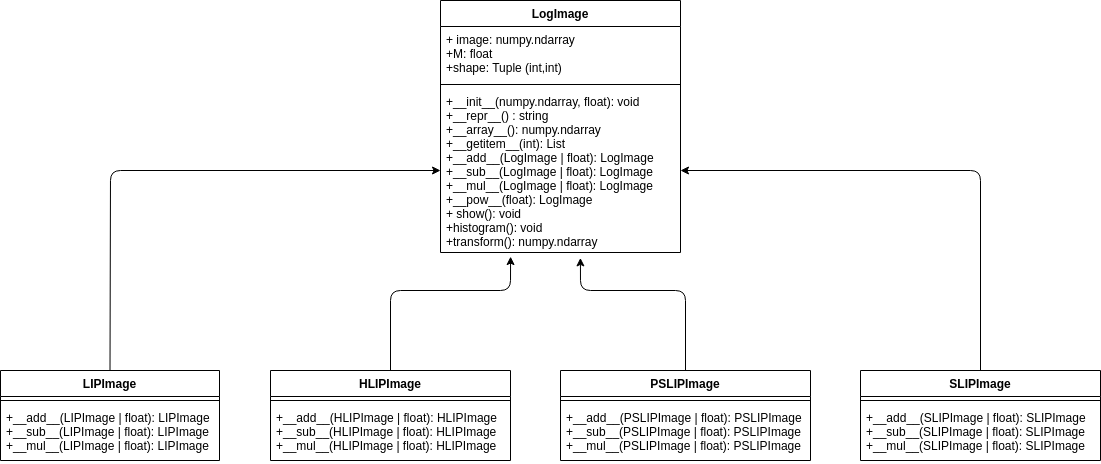
\includegraphics[width=16.0 cm]{images/structures_class_diagram.png}
		\caption{Diagrama de clases de las estructuras no lineales}
	\end{center}
\end{figure}

Para entender mejor la composici\'on del m\'odulo v\'ease el diagrama de clases de la Figura 2.1. Como se puede ver en esta figura se tiene una clase abstracta \verb|LogImage| de la cual heredan las clases \verb|LIPImage|, \verb|HLIPImage|, \verb|PSLIPImage| y \verb|SLIPImage|. Cada una de estas clases representa una imagen en los respectivos modelos: LIP, HLIP, PSLIP y SLIP. Los atributos de la clase padre son:

\begin{itemize}
	\item \verb|M|: el valor de $M$ tal que los niveles de gris de los p\'ixeles de la imagen original se encuentran en el rango $[0,M)$.
	\item \verb|image|: la imagen transformada al espacio de la estructura.
	\item \verb|shape|: una \textit{tupla} de dos enteros que son las dimensiones de la imagen.
\end{itemize}

Adem\'as se definieron los siguientes m\'etodos:

\begin{itemize}
	\item \verb|__init__|: El constructor, que recibe como par\'ametros la imagen original y el valor de $M$ correspondiente. Esta funci\'on en cada una de las diferentes clases transforma la imagen en el espacio original al espacio de la estructura, aplicando primeramente la funci\'on de cambio a tono de gris y luego la funci\'on del isomorfismo.
	\item \verb|__repr__|: Para representar una instancia como un \textit{string} semejante a su atributo \verb|image|.
	\item \verb|__array__|: Que permite que la instancia pueda ser utilizada como un \verb|numpy.ndarray| por las funciones de la librer\'ia \verb|numpy| utilizando su atributo \verb|image|.
	\item \verb|__getitem__|: Que permite indexar una instancia con un entero positivo \verb|i| devolviendo la fila $i$ de la imagen, la cual puede indexarse para acceder a un p\'ixel en espec\'ifico.
	\item \verb|__add__|, \verb|__sub__| y \verb|__mul__|: Que redefinen los operadores \verb|+|, \verb|-| y \verb|*| para la suma, resta y multiplicaci\'on respectivamente. Obs\'ervese que cada una de las clases que heredan de \verb|LogImage| redefinen estos operadores admitiendo solamente para realizar la operaci\'on una instancia de la misma clase, un entero o un n\'umero flotante, dando como salida una nueva instancia de la clase resultado de la operaci\'on realizada. Aclarar que la multiplicaci\'on de dos im\'agenes se hace por parejas de p\'ixeles en la misma posici\'on, diferente a la multiplicaci\'on cl\'asica de matrices.
	\item \verb|__pow__|: Que redefine el operador \verb|**| para elevar la imagen a un escalar $\lambda\in \mathbb{R}$.
	\item \verb|show|: Que lo que hace es mostrar como se ve la imagen en dicho espacio.
	\item \verb|histogram|: Que muestra el histograma de la imagen en dicho espacio.
	\item \verb|transform|: Transforma la imagen al espacio original aplicando la inversa de la funci\'on del isomorfismo y posteriormente la funci\'on de cambio a niveles de grises.
\end{itemize}

Con las clases vistas anteriormente se puede transformar una imagen a otra imagen en el espacio deseado, operar con ella en dicho espacio y luego el resultado regresarlo al espacio original. Obs\'ervese que los espacios parametrizados no se implementaron con estas estructuras, pues estos utilizan diferentes par\'ametros para las diferentes operaciones, algo que no se puede hacer utilizando las estructuras pues una imagen solo se puede transformar de un espacio a otro con un \'unico valor de $M$.

\subsection{Espacios}

\begin{figure}
	\begin{center}
		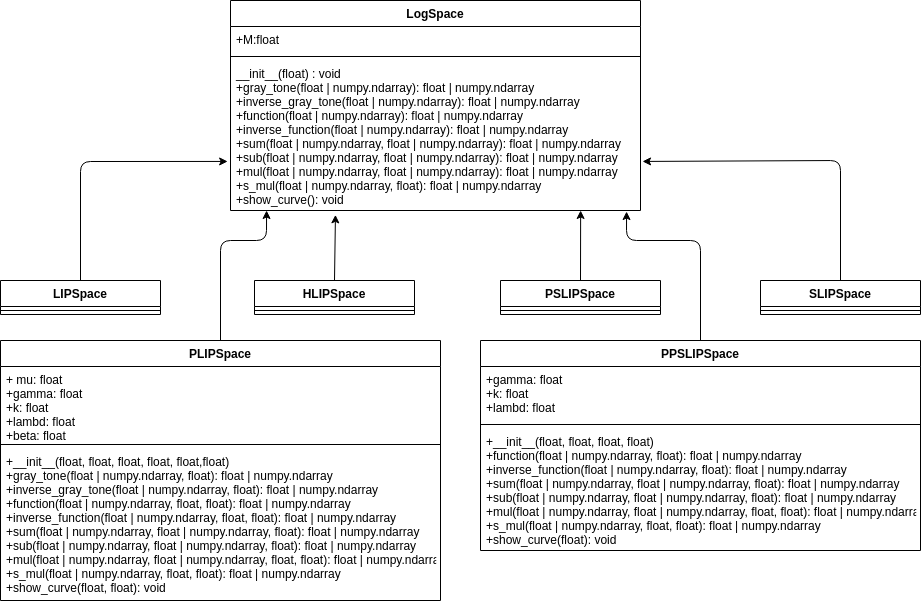
\includegraphics[width=16.0 cm]{images/spaces_class_diagram.png}
		\caption{Diagrama de clases de los espacios no lineales}
	\end{center}
\end{figure}

Para entender mejor la composici\'on del m\'odulo v\'ease el diagrama de clases de la Figura 2.2. Como se puede ver en esta figura se tiene una clase abstracta \verb|LogSpace| de la cual heredan las clases \verb|LIPSpace|, \verb|HLIPSpace|, \verb|PSLIPSpace|, \verb|SLIPSpace|, \verb|PLIPSpace| y \verb|PPSLIPSpace|. Cada una de estas clases contiene las respectivas operaciones de los respectivos modelos: LIP, HLIP, PSLIP, SLIP, PSLIP y PPSLIP. Los atributos de la clase padre son:

\begin{itemize}
	\item \verb|__init__|: El constructor, con el que se inicializa el espacio con un valor de $M$. El espacio PLIP se inicializa adem\'as con los valores de $\mu,~\gamma,~k,~\lambda$ y $\beta$; y por su parte el espacio PPSLIP se inicializa, adem\'as de con el valor de $M$, con los valores de $\gamma,~k$ y $\lambda$.
	\item \verb|gray_tone|: Funci\'on que cambia una imagen o un p\'ixel en niveles de gris a su correspondiente en tonos de gris seg\'un el modelo. Cada uno de los espacios tiene su propia implementaci\'on de esta funci\'on. Los espacios en los que esta funci\'on no se utiliza: SLIP y PPSLIP retornan la imagen sin cambios. Para el caso del espacio PLIP esta tiene un par\'ametro extra para indicar el valor de $\mu$, si este no se especifica se utiliza el valor conque se haya instanciado el espacio.
	\item \verb|inverse_gray_tone|: Inversa de la anterior. Funci\'on que cambia una imagen o un p\'ixel en niveles de gris a su correspondiente en tonos de gris seg\'un el modelo. Para el caso del modelo PLIP tiene un par\'ametro extra para el valor de $\mu$.
	\item \verb|function|: Recibe una imagen o un p\'ixel y devuelve el resultado de aplicarle la funci\'on fundamental del isomorfismo. Se define en cada uno de los espacios. Para los espacios parametrizados la funci\'on puede admitir par\'ametros extras: $\lambda$ y $\beta$ en el caso del PLIP y solo $\lambda$ para el PPSLIP, si no se proporcionan se toman los valores con los que fue instanciado el espacio.
	\item \verb|inverse_function|: Inversa de la funci\'on anterior. Admite los par\'ametros extras para los espacios parametrizados al igual que la funci\'on anterior.
	\item \verb|sum|: Recibe dos im\'agenes o dos p\'ixeles y devuelve la suma de los mismos seg\'un el espacio. Se define en cada espacio. Los espacios parametrizados tienen un par\'ametro extra para pasar un valor de $\gamma$. Si no se proporciona este valor, se utiliza el valor con el que se instanci\'o la clase.
	\item  \verb|sub|: Recibe dos im\'agenes o dos p\'ixeles y devuelve el resultado del primero menos el segundo. Se define en cada espacio. Los espacios parametrizados tienen un par\'ametro extra para pasar un valor de $k$. Si no se proporciona este valor, se utiliza el valor con el que se instanci\'o la clase.
	\item \verb|mul|: Recibe dos im\'agenes o dos p\'ixeles y devuelve la multiplicaci\'on de los mismos seg\'un el espacio. En el caso de las im\'agenes la multiplicaci\'on se hace por parejas de p\'ixeles en la misma posici\'on, diferente a la multiplicaci\'on cl\'asica de matrices. Se define en la clase padre \verb|LogSpace| como $\varphi^{-1}(\varphi(v_1)\cdot\varphi(v-2))$. Los espacios parametrizados redefinen esta funci\'on para poder recibir los par\'ametros y pas\'arselos a \verb|function| y a \verb|inverse_fuction|. Si no se especifican, se utilizan los definidos en el momento de instanciaci\'on del espacio. Esta forma de definici\'on de la multiplicaci\'on aparece en~\cite{panetta2010parameterized} y dado su simpleza se implement\'o de la misma forma en el resto de espacios.
	\item \verb|s_mul|: Recibe una imagen o un p\'ixel y un escalar y devuelve el resultado de la multiplicaci\'on escalar Se define en cada espacio. Los espacios parametrizados tienen un par\'ametro extra para pasar un valor de $\gamma$. Si no se proporciona este valor, se utiliza el valor con el que se instanci\'o la clase.
	\item \verb|show_curve|: Permite visualizar la curva del isomorfismo utilizando el m\'etodo \verb|function| (despu\'es de aplicar la funci\'on de cambio a tono de gris de ser necesario). Se define en cada espacio. Los espacios parametrizados pueden recibir adem\'as los valores de $\lambda$ (PLIP y PPSLIP) y $\beta$ (PLIP). Si no se especifican se utilizan los definidos en el momento de instanciaci\'on del espacio.
\end{itemize}

Con la implementaci\'on de estos espacios se puede trabajar directamente con las im\'agenes como \verb|numpy.ndarray|. Adem\'as de poder utilizar las operaciones b\'asicas, se pueden transformar las im\'agenes utilizando la funci\'on del isomorfismo y utilizar algoritmos para el procesamiento de im\'agenes en dicho espacio. Luego lo obtenido por el algoritmo utilizado se transforma al espacio original para obtener un resultado v\'alido.

\subsection{M\'etricas}

Adem\'as de la EMEE para determinar los mejores par\'ametros en el modelo PLIP, para hacer una comparaci\'on entre las diferentes resultados que arrojan las operaciones y algoritmos de procesamiento de im\'agenes se implement\'o un algoritmo para calcular el contraste promedio de un p\'ixel en una imagen~\cite{patrascu2014mathematical}.

Denotando $p_i =(x_i ,y_i )$, los pares de coordenadas que definen la posición espacial de un píxel en una imagen, el contraste relativo entre dos píxeles distintos $p_1, p_2 \in D$, para una imagen, $f : D \to E$ se define por la relación:

\begin{equation}
	C_R(p_1,p_2)=\frac{1}{d(p_1,p_2)}\cdot\frac{f(p_1)-f(p_2)}{1-\frac{f(p_1)\cdot f(p_2)}{M^2}}
\end{equation}

donde $d(p_1 ,p_2 )$ es la distancia euclidiana entre $p_1$ y $p_2$ en el plano $\mathbb{R}^2$.

Del contraste relativo $C_R$ se define el contraste absoluto como:

\begin{equation}
	C_A(p_1,p_2)=|C_R(p_1,p_2)|=\frac{1}{d(p_1,p_2)}\cdot\frac{|f(p_1)-f(p_2)|}{1-\frac{f(p_1)\cdot f(p_2)}{M^2}}
\end{equation}

Luego de la realizaci\'on de una serie de experimentos se decidi\'o modificar la ecuaci\'on anterior pues esta favorec\'ia a los p\'ixeles de mayor intensidad mucho m\'as que a los p\'ixeles de menor intensidad. V\'ease el siguiente ejemplo.

Supongamos que tenemos dos parejas de p\'ixeles en la cl\'asica escala de enteros de 8 bits: $(p_1,p_2)$ y $(p_3,p_4)$: $f(p_1)=100,~f(p_2)=20,~f(p_3)=230,~f(p_4)=200 \land d(p_1,p_2)=d(p_3,p_4)=t$. Entonces:

\begin{equation}
	C_A(p_1,p_2)=\frac{1}{t}\cdot\frac{|100-20|}{1-\frac{100\cdot20}{256^2}}\approx\frac{82,51}{t}
\end{equation} 

\begin{equation}
	C_A(p_1,p_2)=\frac{1}{t}\cdot\frac{|230-200|}{1-\frac{230\cdot200}{256^2}}\approx\frac{100,63}{t}
\end{equation}

Por tanto $C_A(p_1,p_2)<C_A(p_1,p_2)$ a pesar de que $d(p_1,p_2)=d(p_3,p_4)$ y la diferencia entre la intensidad de $p_1$ y $p_2$ es mucho mayor que la diferencia entre las intensidades de $p_3$ y $p_4$, lo cual en la mayor\'ia de situaciones es incorrecto.

A pesar de esto, la ecuaci\'on (2.10) mostr\'o resultados consecuentes con la calidad de las im\'agenes obtenidas en una gran cantidad de experimentos, pero se mostr\'o deficiente en algunos donde premiaba una imagen m\'as intensa por encima de una menos intensa, en donde claramente se pod\'ia apreciar que la menos intensa ten\'ia una mayor calidad y un mejor contraste. Por este motivo se propuso sustituir la ecuaci\'on (2.10) por la siguiente:

\begin{equation}
	C_A(p_1,p_2)=\frac{|f(p_1)-f(p_2)|}{d(p_1,p_2)}\cdot\frac{256}{M}
\end{equation}

De esta forma el contraste absoluto entre dos p\'ixeles es directamente proporcional a la diferencia de sus intensidades e inversamente proporcional a la distancia entre los mismos, lo cual tiene mucho sentido. El t\'ermino de $\frac{256}{M}$ se utiliza para escalar el resultado de tal forma que se puedan obtener resultados equivalentes, sin importar la escala en que se encuentre una imagen. Esta nueva medida propuesta mostr\'o resultados consecuentes a la calidad de la imagen obtenida tanto en los experimentos en la que la medida definida en (2.10) dio resultados consecuentes como en los que mostr\'o deficiencias.

El contraste para un píxel arbitrario $p \in D$ , para una imagen $f \in F ( D , E )$, se define por la media del contraste absoluto entre el píxel $p$ y los píxeles $( p_i )_{i = 1,...,n}$ que pertenecen a una vecindad $V$. Así tenemos la siguiente fórmula:

\begin{equation}
	\displaystyle C(p)=\frac{1}{n}\sum_{i=1}^{n}C_A(p,p_i)
\end{equation}

Luego de hallado este valor para cada p\'ixel se promedian los resultados para determinar el contraste promedio de un p\'ixel en la imagen denotado por $C_p$.

\subsection{Algoritmos}

\subsubsection{Detecci\'on de Bordes}

La detecci\'on de bordes es uno de los algoritmos m\'as utilizados en el procesamiento de im\'agenes. Para esto se pueden utilizar diferentes filtros como el filtro de Sobel, el filtro de Prewitt, el filtro de Scharr, etc. En particular los tres mencionados anteriormente aparecen implementados en la librer\'ia \verb|skimage.filters| de Python~\cite{module_filters}. En este trabajo se presenta una extensi\'on de estos filtros para utilizarlos con los diferentes modelos no lineales abordados. 

\subsubsection{Unsharp Masking}

\textit{Unsharp Masking} es una t\'ecnica para mejorar la calidad de una imagen. Esta t\'ecnica consiste en determinar los bordes de una imagen y luego fusionar la imagen original con la imagen de bordes de dicha imagen. La fusi\'on m\'as com\'un es la suma lineal, pero pueden existir otras formas de hacer la fusi\'on. En este trabajo se presenta una forma de extensi\'on de este algoritmo utilizando los diferentes modelos no lineales abordados.

\subsubsection{Transformaci\'on Af\'in}

Este algoritmo lo presenta Vasile Pătraşcu en~\cite{patrascu2003gray} donde tambi\'en presenta otro modelo logar\'itmico, pero dada la similitud de este con el HLIP no se aborda en este trabajo.

Consid\'erense estas transformaciones afines en el conjunto de imágenes $F (\Omega, V)$, definidas a continuaci\'on: $\psi : F (\Omega, V ) \to F (\Omega, V )$

\begin{equation}
	\psi(f)=\lambda\otimes(f\oplus\tau)
\end{equation}

donde $\lambda \in \mathbb{R}, \tau \in V y \omega\subset\mathbb{R}^2$ es el soporte de la imagen. Se prefirió usar esta forma porque muestra que una imagen se puede procesar en dos pasos: una traslación de nivel de gris con un valor constante $\tau$ , que conduce a un cambio en el brillo de la imagen, luego una multiplicación escalar con el factor $\lambda$  llevando a un cambio en el contraste de la imagen. Los parámetros $(\lambda, \tau )$ se eligieron de tal manera que se obtuviera una nueva imagen muy cercana (desde un punto de vista estadístico) a una imagen con una distribución uniforme del nivel de gris en el conjunto $V=(a,b)$. Este criterio muestra el hecho de que la imagen mejorada debe tener su media $\mu_u = \frac{a+b}{2}$ y su varianza $\sigma_u^2 = \frac{(b-a)^2}{12}$. De hecho, como resultado, no se est\'a haciendo más que aproximar la transformaci\'on no lineal que produce el algoritmo de ecualización de histogramas de nivel de gris con una transformaci\'on afín como la de (2.15). En estas condiciones para cualquier imagen $f$ con la media $\mu_f$ y la varianza $\sigma_f^2 $, la transformaci\'on afín  se convierte en:

\begin{equation}
	\psi(f)=\frac{\sigma_u}{\sigma_f}\otimes(f\ominus\mu_f)
\end{equation}

Algo muy importante es que este algoritmo solo se puede utilizar en espacios acotados dado que se necesita una cota inferior $a$ y una cota superior $b$ para poder calcular los valores $u_u$ y $\sigma_u^2$ y no puede ocurrir desbordamiento. Bajo estas condiciones solo podemos utilizar los modelos sim\'etricos HLIP y SLIP definidos en los rangos $(-1,1)$ y $(- M, M)$ respectivamente. No se puede utilizar el modelo lineal pues este presenta desbordamiento tanto superior como inferior. El modelo LIP no tiene una cota inferior pues para definir la resta, la escala de gris se expandi\'o a $(-\infty,M)$. En el caso del PSLIP si bien los tonos de gris est\'an acotados en el intervalo real $[0,1)$ para definir la resta de dos p\'ixeles $v_1\ominus v_2$ se exige que $v_1\geq v_2$, lo cual no se garantiza en este algoritmo.

\subsection{Modelo de \textit{Machine Learnig} para Estimar los Par\'ametros en el Modelo PLIP}

Algo en lo que se estuvo trabajando durante el desarrollo de este trabajo fue en la implementaci\'on de un modelo de \textit{Machine Learnig} para estimar de forma r\'apida los mejores par\'ametros, para una determinada operaci\'on del modelo PLIP. Se trabaj\'o en la suma de dos im\'agenes por ser la operaci\'on m\'as b\'asica de todas. La idea era que dadas dos im\'agenes cualesquiera el modelo fuera capaz de detectar con que par\'ametros de $\gamma(M)$ y $\mu(M)$ se obten\'ia una mejor imagen para la suma de las im\'agenes dadas de entrada.

La idea fue utilizar una red convolucional, ya que es conocido que estas son el mejor modelo para el an\'alisis de im\'agenes. El modelo implementado fue una red neuronal muy sencilla basada en la arquitectura de Lenet-5 propuesta por Yann LeCun en 1998. A grandes rasgos, la red propuesta se compon\'ia de una capa convolucional, seguida de una capa de \textit{max-pooling}, seguida esta a su vez de otra capa convolucional y otra capa de \textit{max-pooling}. Las capas convolucionales ten\'ian como funci\'on de activaci\'on a ``ReLu''. Luego se aplana el volumen resultante utilizando una capa \verb|Flaten|, seguido de esta una red neuronal de dos capas cada una con funci\'on de activaci\'on ``ReLu'' y finalmente la capa de salida con funci\'on de activaci\'on ``softmax''. La cantidad de neuronas en esta \'ultima capa correspond\'ia a la cantidad de categor\'ias en las que se dividieron a las im\'agenes. El tama\~no del \textit{kernel} y la cantidad de filtros en las capas convolucionales y la cantidad de neuronas en las antepen\'ultima y pen\'ultima capa se variaron en busca de obtener mejores resultados.

Para la confecci\'on del conjunto de datos, se utilizaron parejas de im\'agenes de diferentes dimensiones, eso s\'i las im\'agenes de una misma pareja s\'i ten\'ian la misma dimensi\'on. Los mejores valores de $\gamma(M)$ y $\mu(M)$ se estimaron para cada pareja utilizando como mediada la EMEE. Luego las im\'agenes fueron divididas por categor\'ias de tipo $(\gamma(M),\lambda(M))$. Como el modelo solo puede analizar una imagen y no parejas de ellas, cada pareja se fusion\'o en una sola imagen de modo que una imagen quedaba encima de la otra bordeadas y separadas entre ellas por valores de intensidad cero de tal forma que al final todas las fusiones de parejas tuvieran la misma dimensi\'on. Esto por supuesto llev\'o a que en una fusi\'on las im\'agenes quedaran m\'as bordeadas y separadas que en otra, en dependencia de las dimensiones de las im\'agenes que compon\'ian la fusi\'on.

Luego de tener las im\'agenes fusionadas divididas en los diferentes grupos, se procedi\'o a entrenar el modelo con un grupo de las mismas, mientras que otro grupo se dej\'o para evaluar los resultados. Finalmente el mayor resultado que se obtuvo fue de un $55\%$ de acierto, lo cual no es muy bueno. Debido a la falta de tiempo y al no abundante conocimiento por parte del autor de este tipo de modelos, finalmente la presentaci\'on de esta propuesta fue descartada. Sin embargo esta idea no deber\'ia ser abandona pues un estudio m\'as profundo podr\'ia dar buenos resultados. Quiz\'as modificaciones en el modelo, la utilizaci\'on de otras m\'etricas para obtener los par\'ametros, un mejor conjunto de datos, una mejor forma de realizar las fusiones o incluso la utilizaci\'on de otro modelo son alternativas que podr\'ian conllevar a la obtenci\'on de buenos resultados en la estimaci\'on de dichos par\'ametros de forma eficiente.
\chapter{Detalles de Implementación y Experimentos}\label{chapter:implementation}

\section{Detalles de implementaci\'on}

En esta secci\'on se abordar\'an algunos detalles que se tuvieron en cuenta a la hora de implementar este m\'odulo.

\subsection{Modelos}

Primeramente obs\'ervese que el rango de niveles de gris de una imagen se define como $[0,M)$. Por ende al transformar la imagen a una funci\'on de tono de gris utilizando la f\'ormula (1.11) cuando el nivel de gris es 0 el tono de gris es $M$, lo cual contradice que el rango de tono de gris para el modelo LIP es $[0,M)$. Por este motivo tanto para la clase \verb|LIPImage| como \verb|LIPSpace| antes de cambiar la imagen de niveles de gris a tonos de gris, esta primero se procesa de tal forma que el menor valor admisible sea un n\'umero cercano a cero, pero mayor que este. En esta implementaci\'on se decidi\'o utilizar el n\'umero $0.0001$. No se opt\'o por otras alternativas como por ejemplo el \'epsilon de la m\'aquina porque al realizar operaciones aritm\'eticas este valor se convert\'ia en cero y por ende no solucionaba el problema planteado. Esto tambi\'en se hizo en la implementaci\'on del modelo PLIP. Para el caso del modelo SLIP no fue necesario pues no se utiliza una funci\'on de cambio a tono de gris y se trabaja directamente con los niveles de gris.

Otro problema que fue necesario resolver es que en el modelo HLIP los niveles de gris de la imagen a transformar deben estar en el rango $(0,M)$. La soluci\'on propuesta fue hacer algo similar al caso anterior.

Las implementaciones de todos los modelos tal y como se explic\'o en el cap\'itulo anterior se pueden encontrar en el subm\'odulo ``models'', cada uno en su archivo correspondiente.

\subsection{M\'etricas}

Como se explic\'o en el cap\'itulo exterior se implementaron dos m\'etricas: EMEE y $C_p$. La implementaci\'on de estas m\'etricas se puede encontrar en el subm\'odulo ``metrics''. Este subm\'odulo consta de dos archivos: ``emee.py'' y ``contrast\_pixel''. 

\subsubsection{EMEE}
En el archivo ``emee.py'' se encuentran dos funciones: \verb|emee| y \verb|find_min_max|. La primera devuelve el valor de EMEE de una imagen dada como entrada. Adem\'as recibe como par\'ametros el valor de $\alpha$, las dimensiones de los bloques en los que se desea dividir la imagen y una constante $c$. Esta constante se utiliza para evitar la divisi\'on por $0$ en (1.33). Se suma tanto al numerador como al denominador de las fracciones que aparecen. La constante que se utiliz\'o para calcular los mejores par\'ametros fue $0.5$. Esto tambi\'en para evitar que una divisi\'on por un n\'umero muy cercano a 0 diera un resultado demasiado grande. 

La funci\'on \verb|find_min_max| se utiliza para calcular el menor y mayor valor de intensidad de un bloque. Da como salida una \textit{tupla} con dichos valores en ese orden y recibe una imagen y 4 enteros: $n_1,n_2,m_1,m_2$, tal que $(n_1,m_1)$ son las coordenadas donde inicia el bloque y; $n_2$ y $m_2$ son la dimensi\'on horizontal y vertical del bloque respectivamente.

\subsubsection{Contraste Promedio}
En el archivo ``contrast\_pixel.py'' se encuentran tres funciones. La primera funci\'on \verb|abs_contrast_2_pixels| se utiliza para calcular el contraste absoluto entre 2 p\'ixeles. Recibe dos \textit{tuplas} de 3 elementos, tal que cada una representa representa un p\'ixel (las coordenadas y el valor de intensidad del p\'ixel), y el valor de $M$.  La segunda funci\'on \verb|contras_pixel| calcula el contraste de un p\'ixel en una imagen; recibe como par\'ametros una \textit{tupla} que representa al p\'ixel, la imagen, el valor de $M$ y un valor $v$ que indica el radio de la vecindad a considerarse. 

La \'ultima funci\'on \verb|contrast_img| da como salida el contraste promedio de un p\'ixel en una imagen, o sea $C_p$. Esta funci\'on recibe como par\'ametros la imagen, el valor de $M$ y el radio de la vecindad que se debe tener en cuenta alrededor de un p\'ixel. Como calcular el contraste para cada p\'ixel de una imagen es un proceso que puede demorar seg\'un el tama\~no de la imagen, se tom\'o la decisi\'on de, para im\'agenes cuya resoluci\'on fuese mayor que $300\times300$, escoger un subconjunto de p\'ixeles. El criterio para escoger dichos p\'ixeles fue el siguiente:

\begin{enumerate}
	\item Iniciar desde la posici\'on $(0,0)$
	\item Si se analiz\'o el p\'ixel en la posici\'on $(i,j)$ el pr\'oximo p\'ixel a analizar es el p\'ixel $(i,j+3)$
	\item Una vez terminada de analizar una fila $i$ la pr\'oxima fila a analizar es la fila $i+3$.
\end{enumerate}

El radio de la vecindad que se tom\'o para calcular el contraste de cada p\'ixel fue de 2. Al comparar ambas formas se pudo comprobar que, para im\'agenes con una resoluci\'on grande, la forma propuesta, reduce considerablemente el tiempo de ejecuci\'on, afectando en una cantidad despreciable el resultado final.

\subsection{Algoritmos}

La implementaci\'on de los algoritmos explicados en el cap\'itulo anterior se encuentra en el subm\'odulo ``algorithms''. Este subm\'odulo se compone de tres archivos: ``edge\_detection'', ``unsharp\_masking'' y ``affine\_transform.py''.

\subsubsection{Detecci\'on de Bordes}

El archivo ``edge\_detection'' tiene implementadas dos funciones: \verb|edge_detection| y \verb|space_edge_detection|. La primera recibe como par\'ametros una imagen y un filtro y da como salida el resultado de aplicarle el filtro a la imagen. 

La segunda funci\'on, adem\'as de recibir estos mismos par\'ametros, recibe una instancia de tipo \verb|LogSpace|. Esta se utiliza para indicar el modelo que se desea a utilizar. El funcionamiento es sencillo: se transforma la imagen al isomorfismo utilizando primeramente la funci\'on de cambio a tonos de gris y luego la funci\'on del isomorfismo, se aplica el filtro a la imagen transformada y se regresa este resultado al espacio original utilizando primero la inversa de la funci\'on del isomorfismo y luego la funci\'on de cambio a niveles de gris. Recu\'erdese que los modelos que no utilizan funciones de cambio, en su implementaci\'on, dan como salida la misma imagen dada de entrada.

\subsubsection{Unsharp Masking}

El archivo ``unsharp\_masking.py'' consta de dos funciones: \verb|unsharp_masking| y \verb|space_unsharp_masking|. La primera recibe como par\'ametros una imagen, un filtro y un \textit{string} que puede ser: \verb|``+''| o \verb|``-''|. La salida de esta funci\'on es el resultado de utilizar el filtro para detectar los bordes de la imagen y fusionar la imagen original y la imagen de bordes utilizando la suma (\verb|``+''|) o la resta (\verb|``-''|) lineal. 

La segunda funci\'on, adem\'as de recibir estos mismos par\'ametros, recibe una instancia de tipo \verb|LogSpace|. Este algoritmo primero transforma la imagen al isomorfismo utilizando primeramente la funci\'on de cambio a tonos de gris y luego la funci\'on del isomorfismo, se aplica el filtro dado y luego seg\'un el operador especificado, a la imagen original se le suma o se le resta la imagen de bordes. Finalmente se utilizan la inversa de la funci\'on del isomorfismo y la funci\'on de cambio a niveles de gris para regresar al espacio original. El permitir que la que fusi\'on, adem\'as de con la suma se haga con la resta, se tom\'o como decisi\'on despu\'es de que uno de los modelos mostr\'o buenos resultados utilizando la resta en lugar de la suma. 

\subsubsection{Transformaci\'on Af\'in}

El archivo ``affine\_transform.py'' contiene a \verb|space_affine_transform| como \'unica funci\'on definida. Esta funci\'on da como salida la transformaci\'on af\'in explicada en el cap\'itulo anterior utilizando las operaciones aritm\'eticas de un modelo espec\'ifico. Recibe como par\'ametros una imagen, los extremos del intervalo en el cual se va a realizar la transformaci\'on y una instancia de tipo \verb|LogSpace|. Este \'ultimo par\'ametro se utiliza para indicar con que modelo se quiere realizar la transformaci\'on. Los extremos del intervalo de entrada deben ser los del modelo utilizado para obtener los mejores resultados.

\section{Experimentos}
Para los experimentos que a continuaci\'on se muestran se utilizaron im\'agenes en escala de gris de 8 bits, o sea que los valores de intensidades de los p\'ixeles eran n\'umeros enteros en el intervalo $[0,255]$. Aqu\'i es importante aclarar que los modelos trabajan y dan resultados utilizando n\'umeros de tipo \textit{float64}. Para el mostrado y guardado de las im\'agenes \verb|skimage| primero rescala las im\'agens a n\'umeros flotantes entre $[0,1]$ haciendo \textit{stretching} utilizando como extremos los valores de menor y mayor intensidad presentes en la imagen. Luego esta se lleva a la escala de enteros de 8 bits para mostrar y guardar la imagen~\cite{image_data_types_and_what_they_mean}.

Para la realizaci\'on de un an\'alisis estad\'isticos se confeccionaron tres \text{datasets} de im\'agenes. El primero se compone de varias im\'agenes naturales separadas en diferentes grupos, tal que si dos im\'agenes pertenecen a un mismo grupo, estas tienen la misma resoluci\'on. Estas im\'agenes se utilizaron para el experimento de la suma, donde las im\'agenes de un mismo grupo se sumaron utilizando los diferentes modelos. En toral se formaron 774 parejas. El segundo \textit{dataset} es un conjunto de 200 im\'agenes naturales. El tercer \textit{dataset} es un conjunto de 200 im\'agenes m\'edicas de radiograf\'ias de t\'orax tanto de frente como de perfil. Estos dos \'ultimos \textit{datasets} se utilizaron para el estudio de los diferentes algoritmos utilizando los diferentes modelos.

En cada uno de los diferentes experimentos primero se muestran y analizan dos ejemplos y luego se presentan las estad\'isticas del estudio realizado.

\subsection{Curvas de los isomorfismos}
Lo primero que se muestra son las curvas de los diferentes isomorfismos, iniciando por los no parametrizados que se muestran en la Figura 3.1. Para los isomorfismos LIP y PSLIP se muestra adem\'as los puntos respectivos a los valores: 0 (rojo), 128 (naranja) y 255(amarillo). Para el caso de HLIP se muestran los puntos para los valores: 1 (rojo), 128 (naranja) y 255 (amarillo). Para el caso del modelo SLIP se muestran los puntos para los valores: -255 (morado) -128(verde) 0 (rojo), 128 (naranja) y 255(amarillo).

\begin{figure}
	\begin{center}
		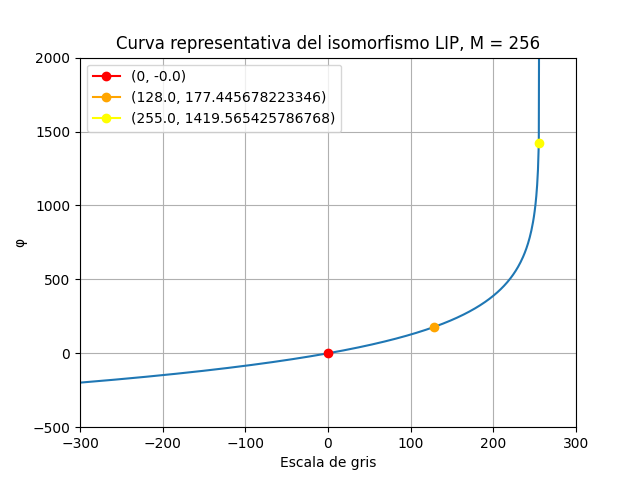
\includegraphics[width=5.5 cm]{images/clasics_curves/lip_curve.png}
		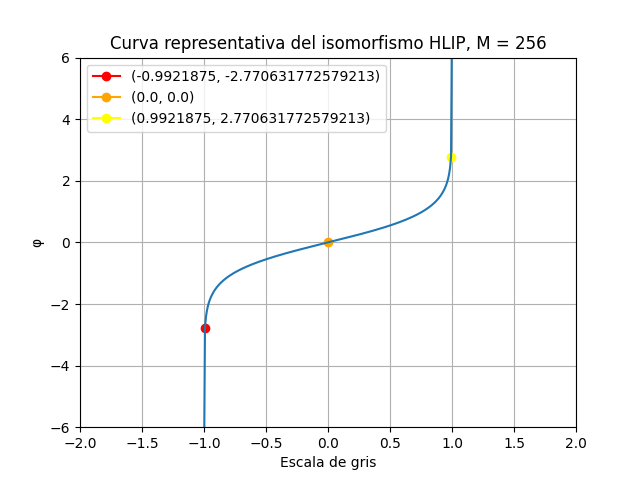
\includegraphics[width=5.5 cm]{images/clasics_curves/hlip_curve.png}
		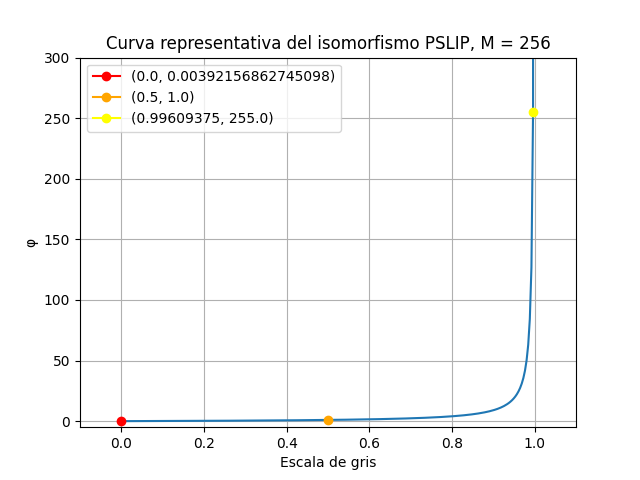
\includegraphics[width=5.5 cm]{images/clasics_curves/pslip_curve.png}
		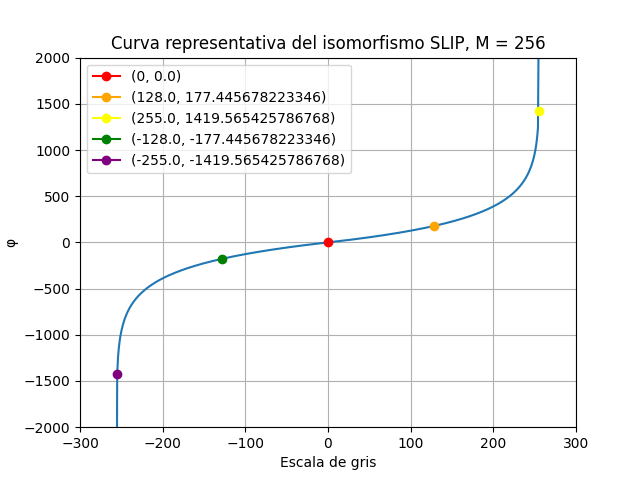
\includegraphics[width=5.5 cm]{images/clasics_curves/slip_curve.png}
		\caption{Curvas representativas de los modelos no parametrizados}
	\end{center}
\end{figure}

En las Figura 3.2 y Figura 3.3 se pueden observar varias curvas del modelo PLIP y PPSLIP utilizando diferentes valores de $\lambda(M)$. En ambos modelos se puede apreciar la tendencia a la linealidad a medida que el valor de $\lambda(M)$ aumenta. Obs\'ervese que los puntos correspondiente a 0 (rojo), 128 (naranja) y 255 (amarillo) se van acercando a una l\'inea recta. Tambi\'en se muestra que los nuevos valores que aparecen siguen manteniendo la estructura logar\'itmica.

\begin{figure}
	\begin{center}
		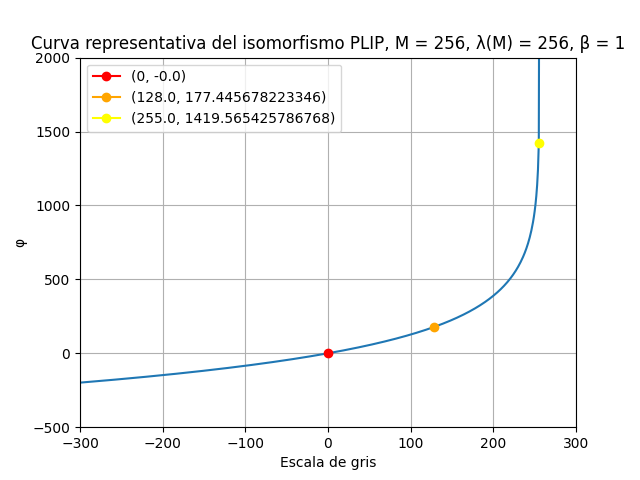
\includegraphics[width=5.5 cm]{images/plip_curves/plip_curve_256.png}
		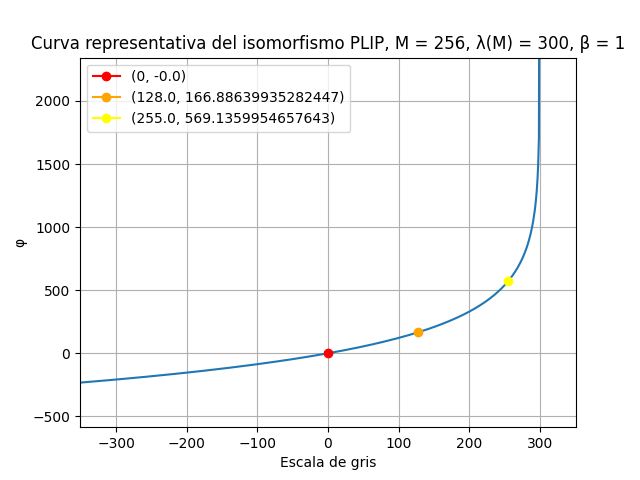
\includegraphics[width=5.5 cm]{images/plip_curves/plip_curve_300.png}
		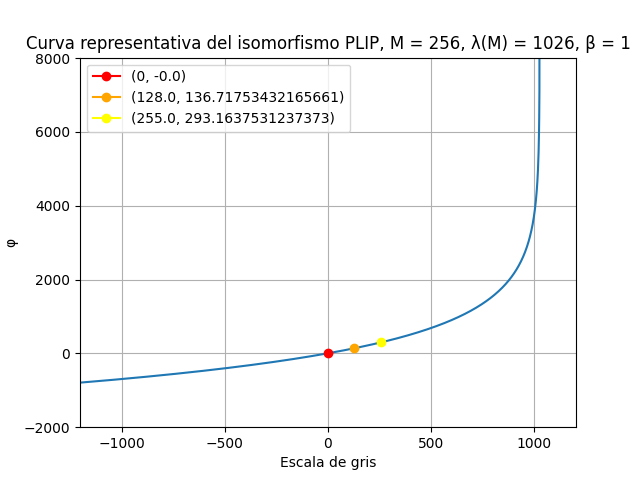
\includegraphics[width=5.5 cm]{images/plip_curves/plip_curve_1026.png}
		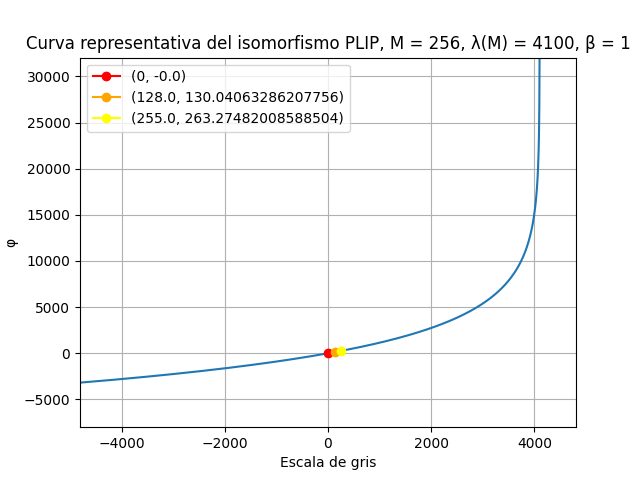
\includegraphics[width=5.5 cm]{images/plip_curves/plip_curve_4100.png}
		\caption{Curvas representativas del modelo PLIP con diferentes valores de $\lambda(M)$}
	\end{center}
\end{figure}

\begin{figure}
	\begin{center}
		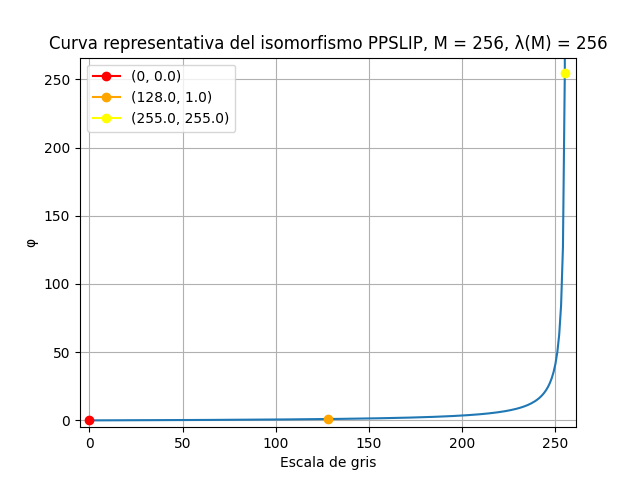
\includegraphics[width=5.5 cm]{images/ppslip_curves/ppslip_curve_256.png}
		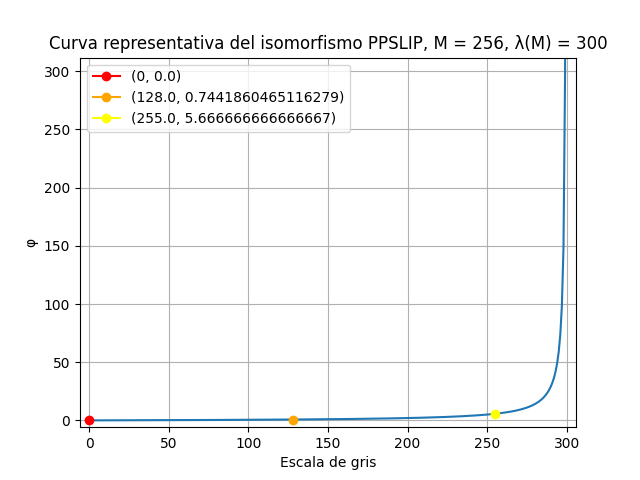
\includegraphics[width=5.5 cm]{images/ppslip_curves/ppslip_curve_300.png}
		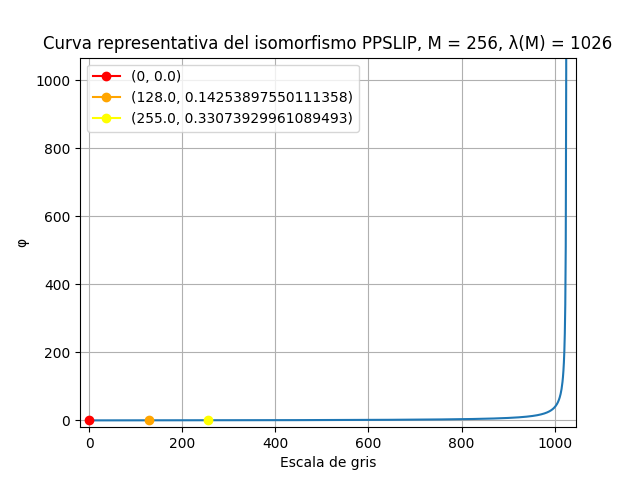
\includegraphics[width=5.5 cm]{images/ppslip_curves/ppslip_curve_1026.png}
		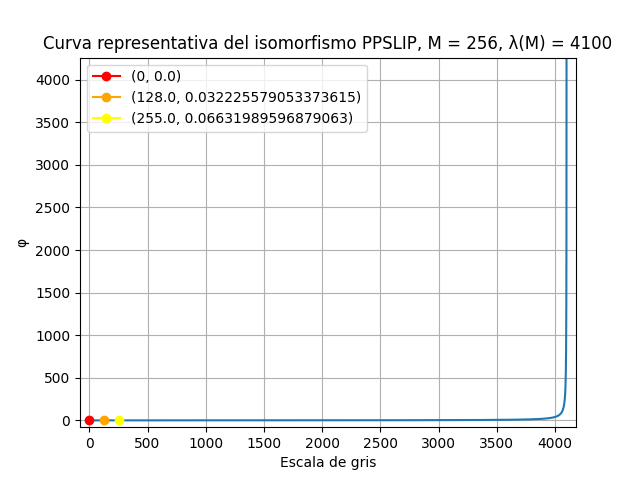
\includegraphics[width=5.5 cm]{images/ppslip_curves/ppslip_curve_4100.png}
		\caption{Curvas representativas del modelo PPSLIP con diferentes valores de $\lambda(M)$}
	\end{center}
\end{figure}

\subsection{Suma de im\'agenes}

\subsubsection{Ejemplos}

Una de las formas m\'as utilizadas para la fusi\'on de im\'agenes es la suma de las mismas. Para los ejemplos que se muestran a continuaci\'on se utilizaron las im\'agenes: Playa, Patineta, Monta\~na e Insecto que se muestran en la Figura 3.4.

\begin{figure}
	\begin{center}
		\subfigure[Playa]{
		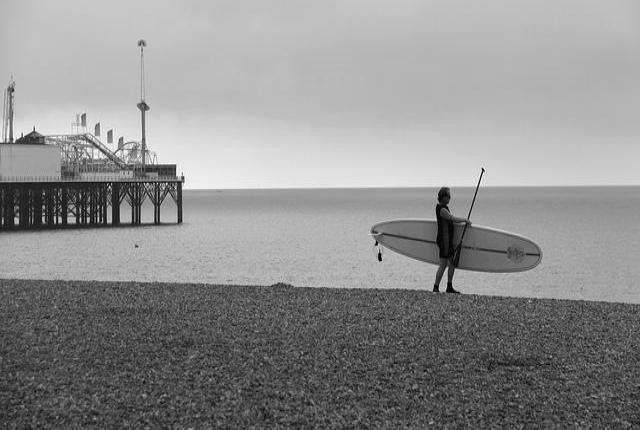
\includegraphics[width=5.5 cm]{images/originals/playa.jpg}}
		\subfigure[Patineta]{
			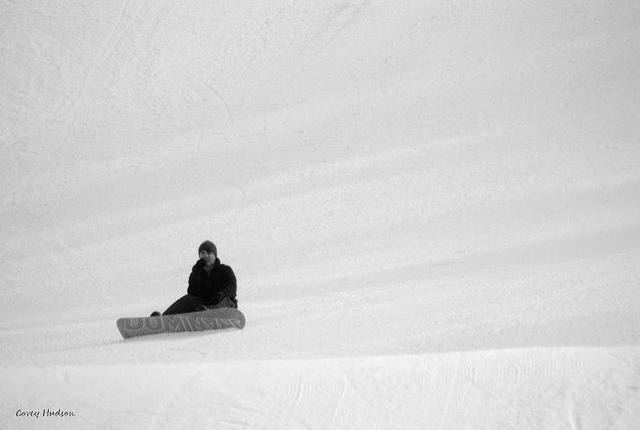
\includegraphics[width=5.5 cm]{images/originals/patineta.jpg}}
		\subfigure[Monta\~na]{
			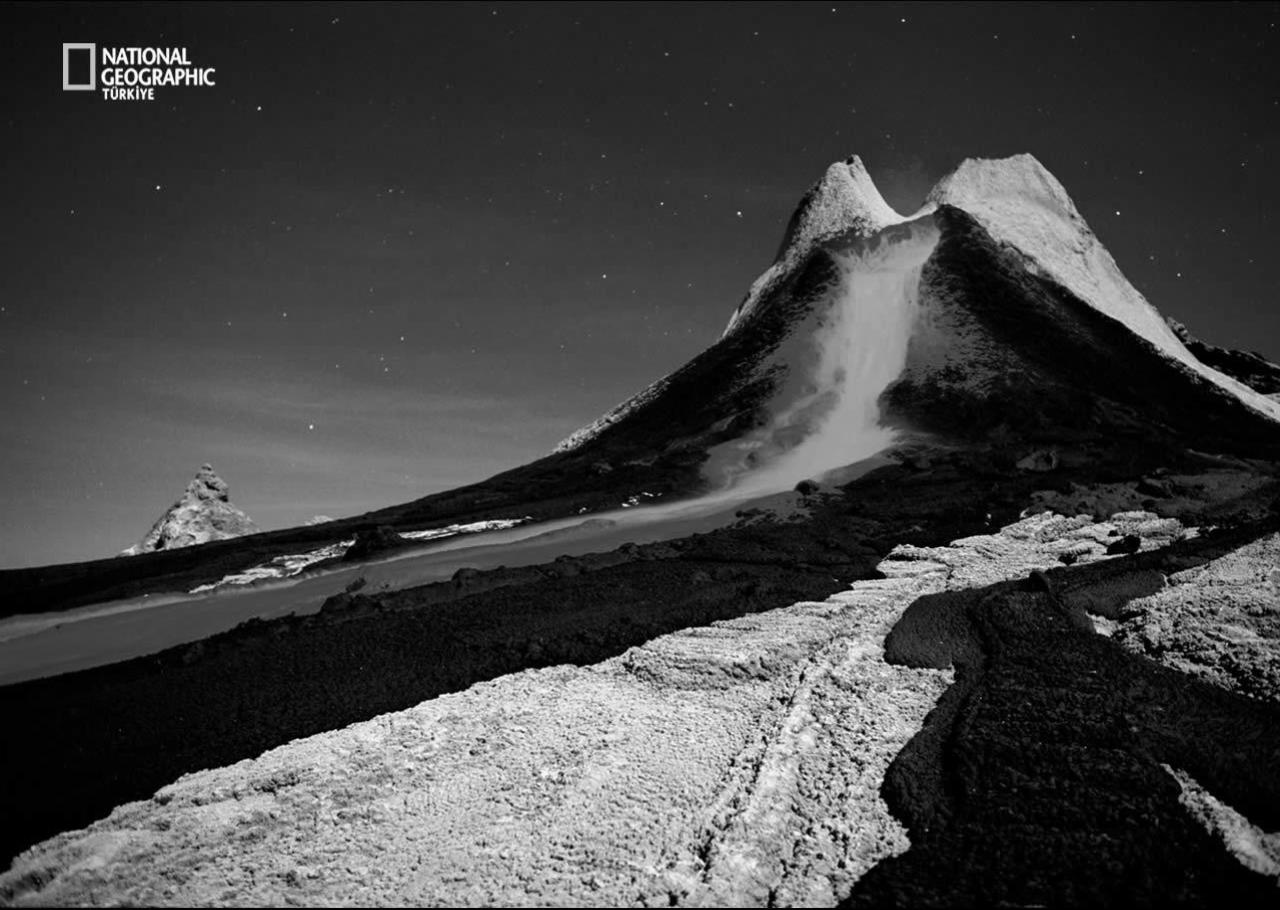
\includegraphics[width=5.5 cm]{images/originals/montania.jpg}}
		\subfigure[Insecto]{
			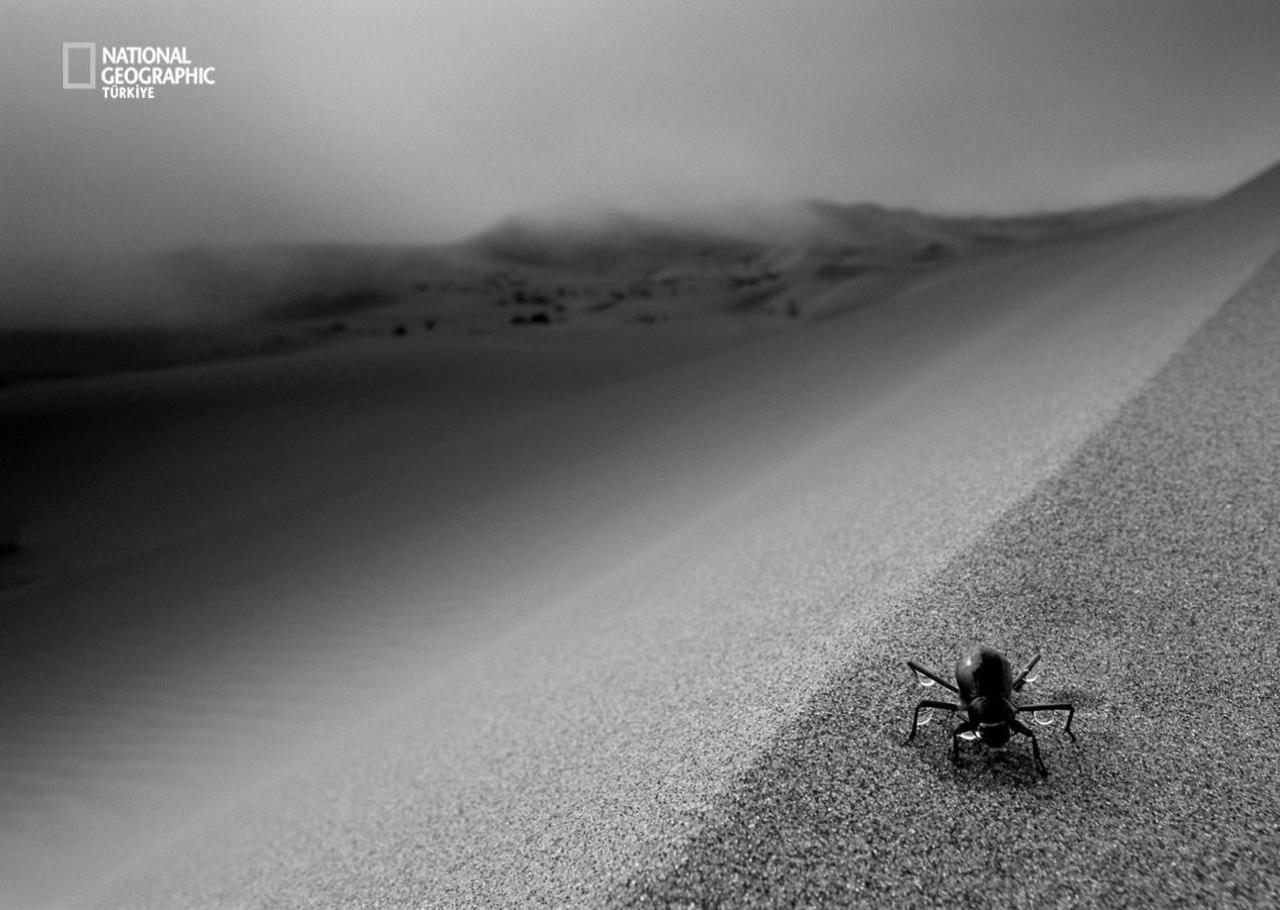
\includegraphics[width=5.5 cm]{images/originals/insecto.jpg}}
		\caption{Im\'agenes para los experimentos de suma}
	\end{center}
\end{figure}

\begin{figure}
	\begin{center}
		\subfigure[Lineal $C_p=3.49$]{
			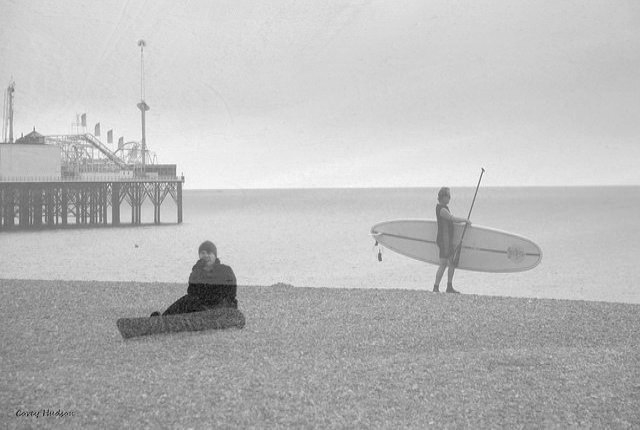
\includegraphics[width=5.5 cm]{images/sums/p y p/sab.png}}
		\subfigure[LIP $C_p=5.71$]{
			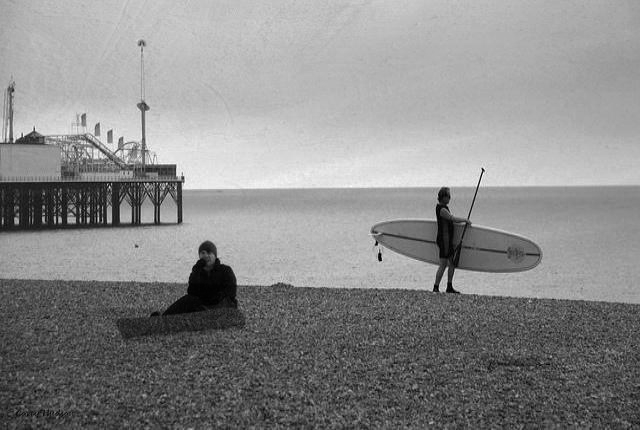
\includegraphics[width=5.5 cm]{images/sums/p y p/jsab.png}}
		\subfigure[HLIP $C_p=4.96$]{
			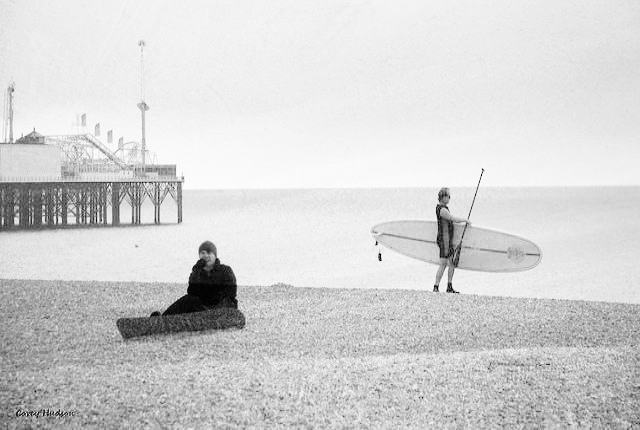
\includegraphics[width=5.5 cm]{images/sums/p y p/hsab.png}}
		\subfigure[PSLIP $C_p=1.39$]{
			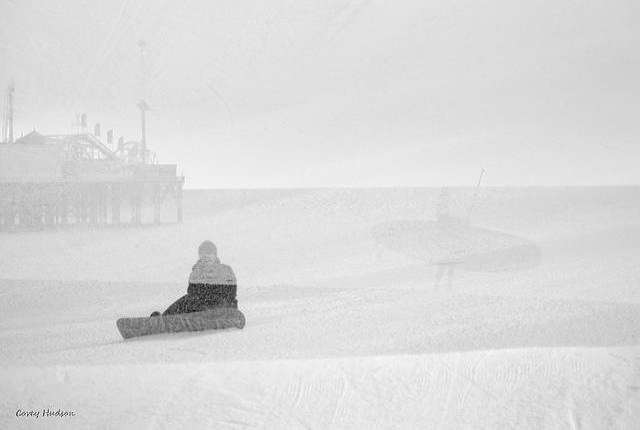
\includegraphics[width=5.5 cm]{images/sums/p y p/pssab.png}}
		\subfigure[SLIP $C_p=1.45$]{
			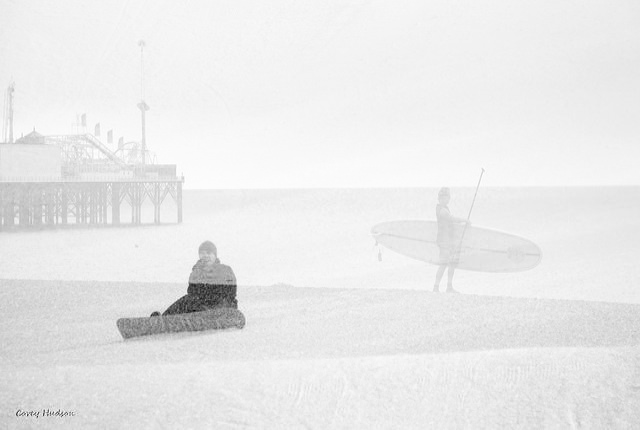
\includegraphics[width=5.5 cm]{images/sums/p y p/ssab.png}}
		\subfigure[PLIP $C_p=5.71$]{
			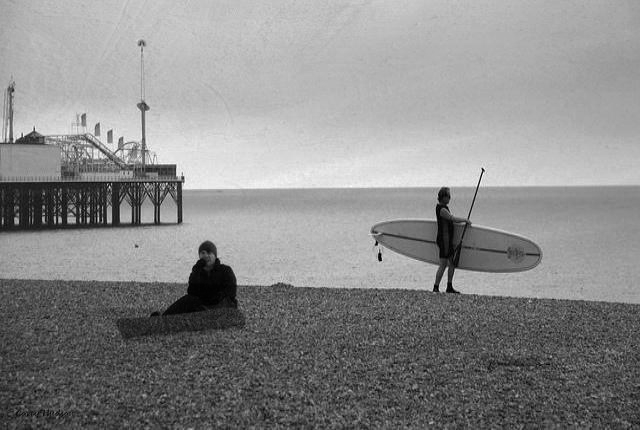
\includegraphics[width=5.5 cm]{images/sums/p y p/psab.png}}
		\subfigure[PPSLIP $C_p=3.35$]{
			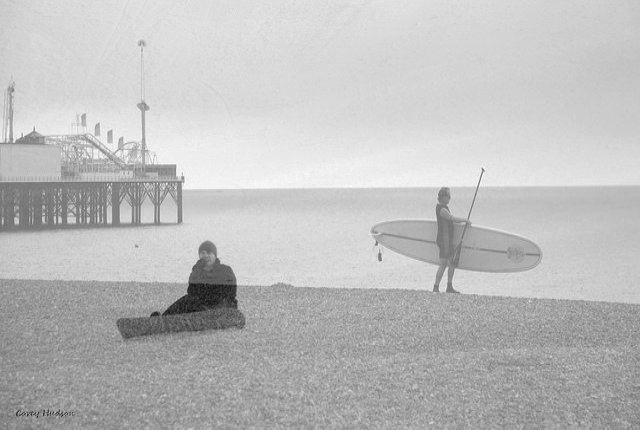
\includegraphics[width=5.5 cm]{images/sums/p y p/ppssab.png}}
		\caption{Suma de Playa y Patineta utilizando los diferentes modelos}
	\end{center}
\end{figure}

\begin{figure}
	\begin{center}
		\subfigure[Lineal $C_p=3.15$]{
			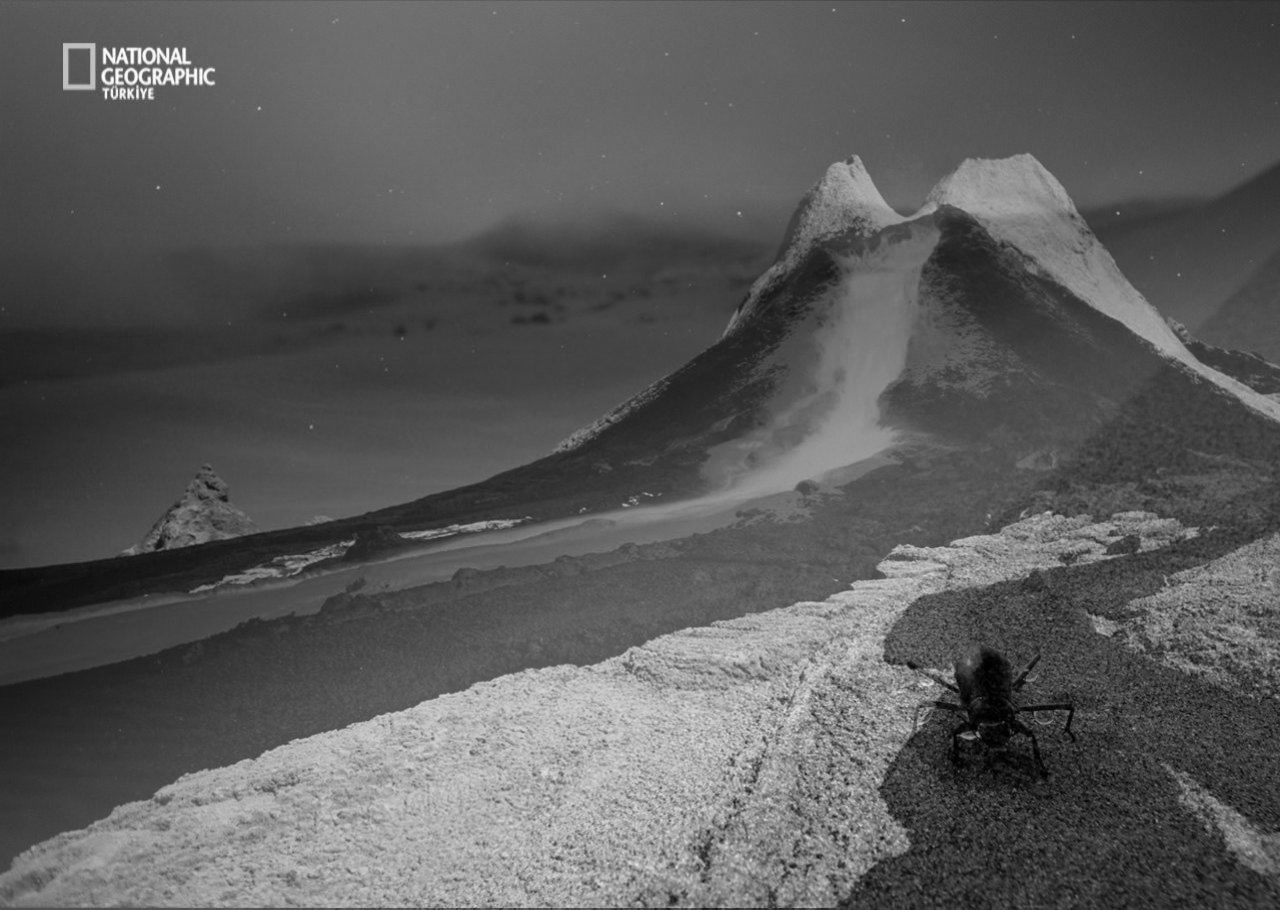
\includegraphics[width=5.5 cm]{images/sums/m y i/scd.png}}
		\subfigure[LIP $C_p=2.77$]{
			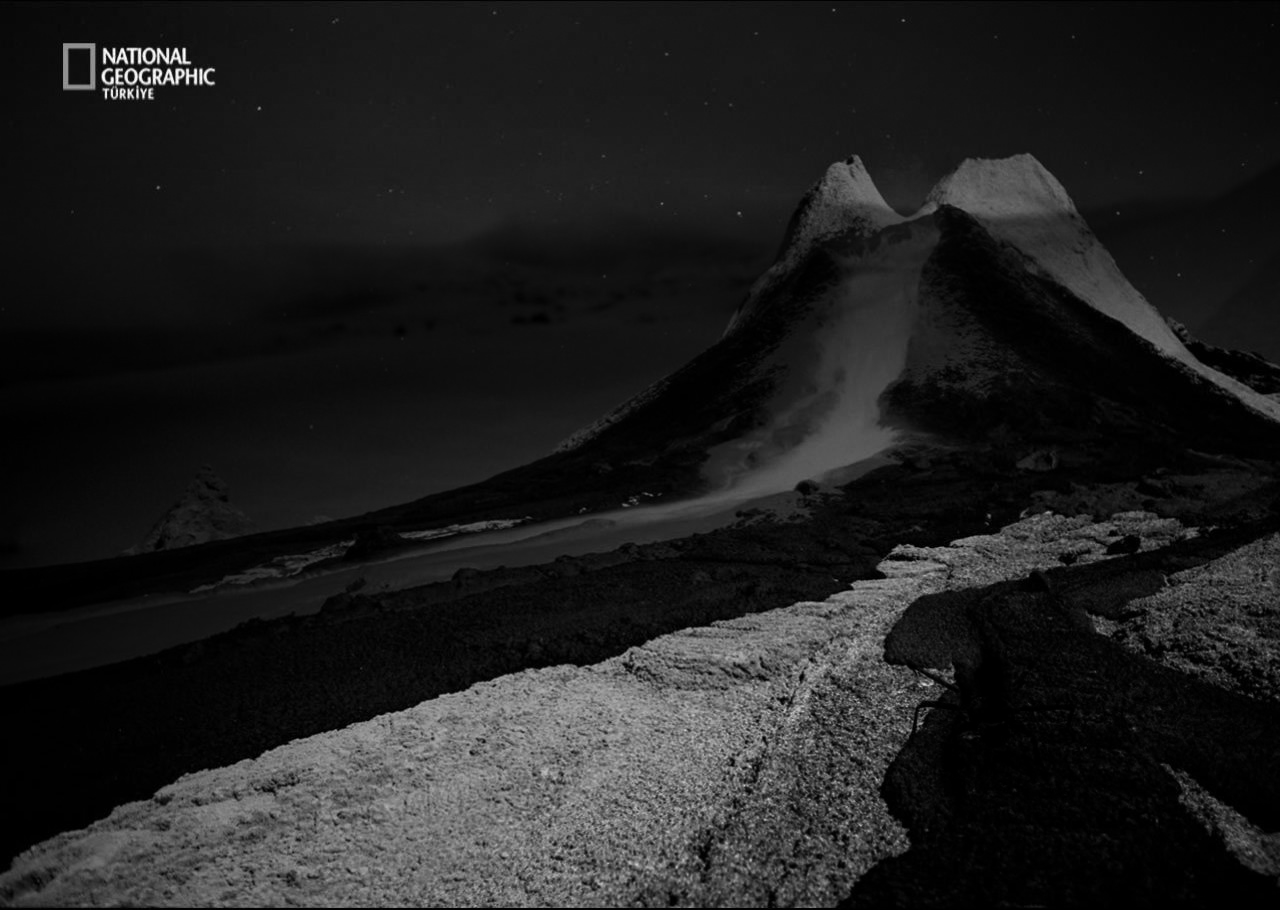
\includegraphics[width=5.5 cm]{images/sums/m y i/jscd.png}}
		\subfigure[HLIP $C_p=4.53$]{
			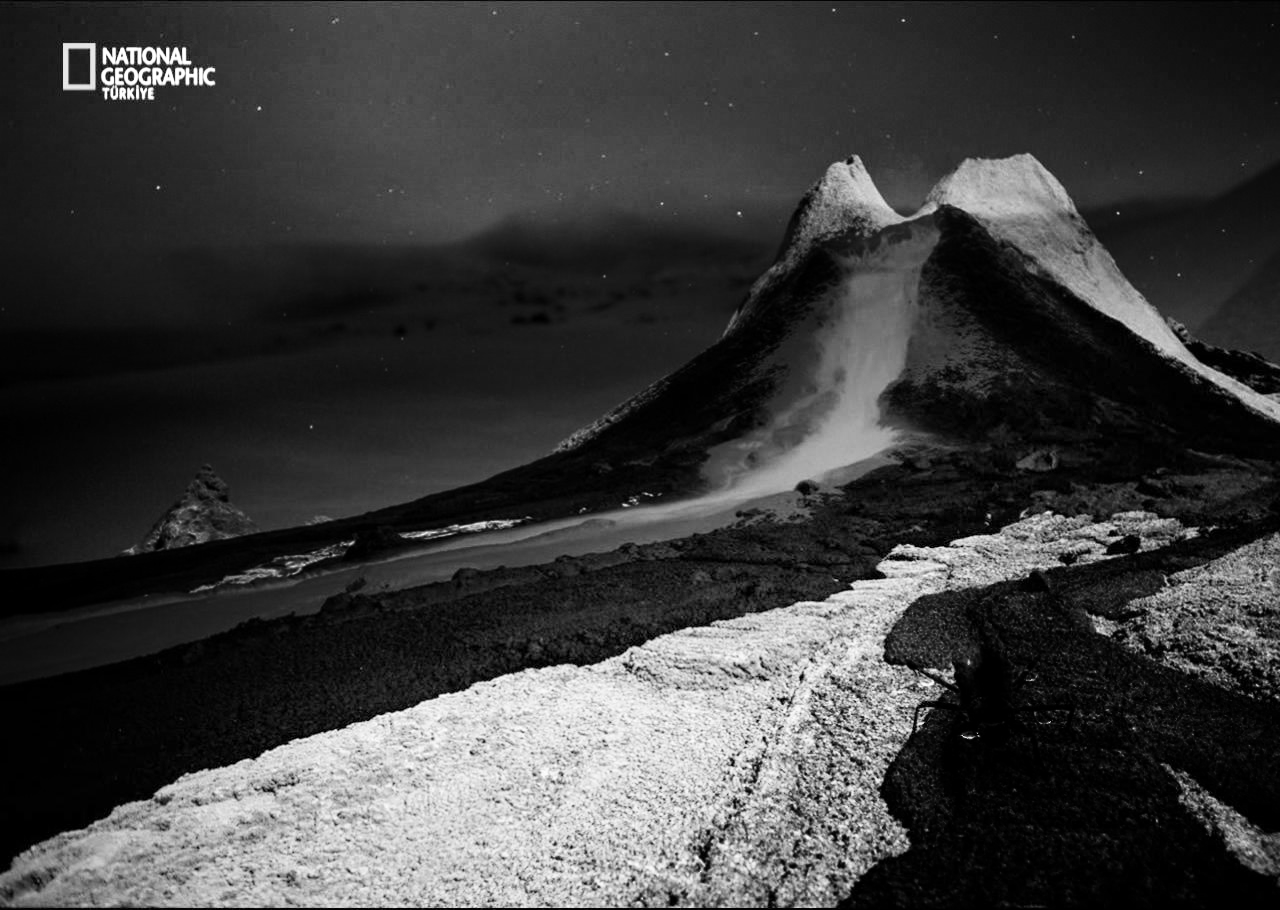
\includegraphics[width=5.5 cm]{images/sums/m y i/hscd.png}}
		\subfigure[PSLIP $C_p=3.47$]{
			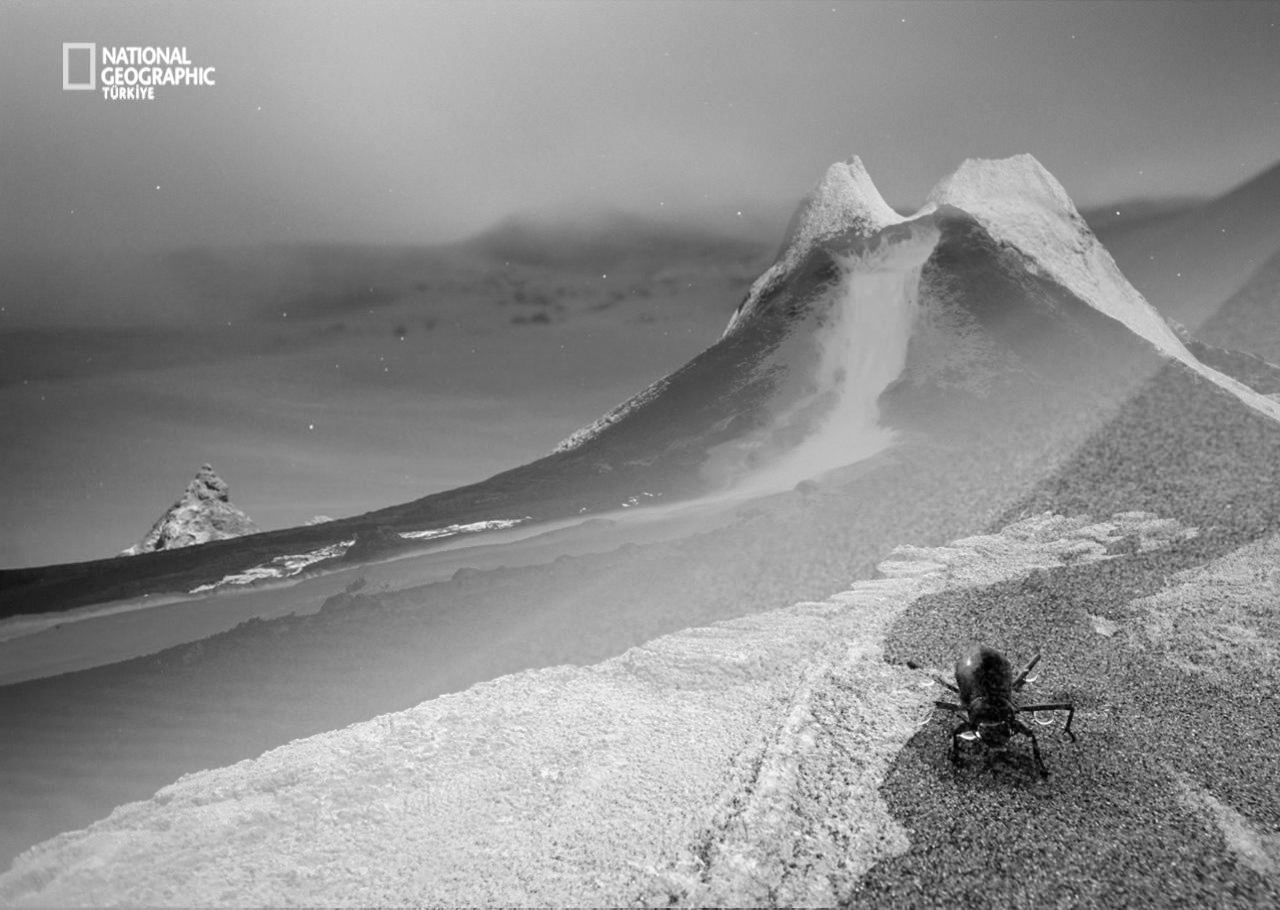
\includegraphics[width=5.5 cm]{images/sums/m y i/psscd.png}}
		\subfigure[SLIP $C_p=3.65$]{
			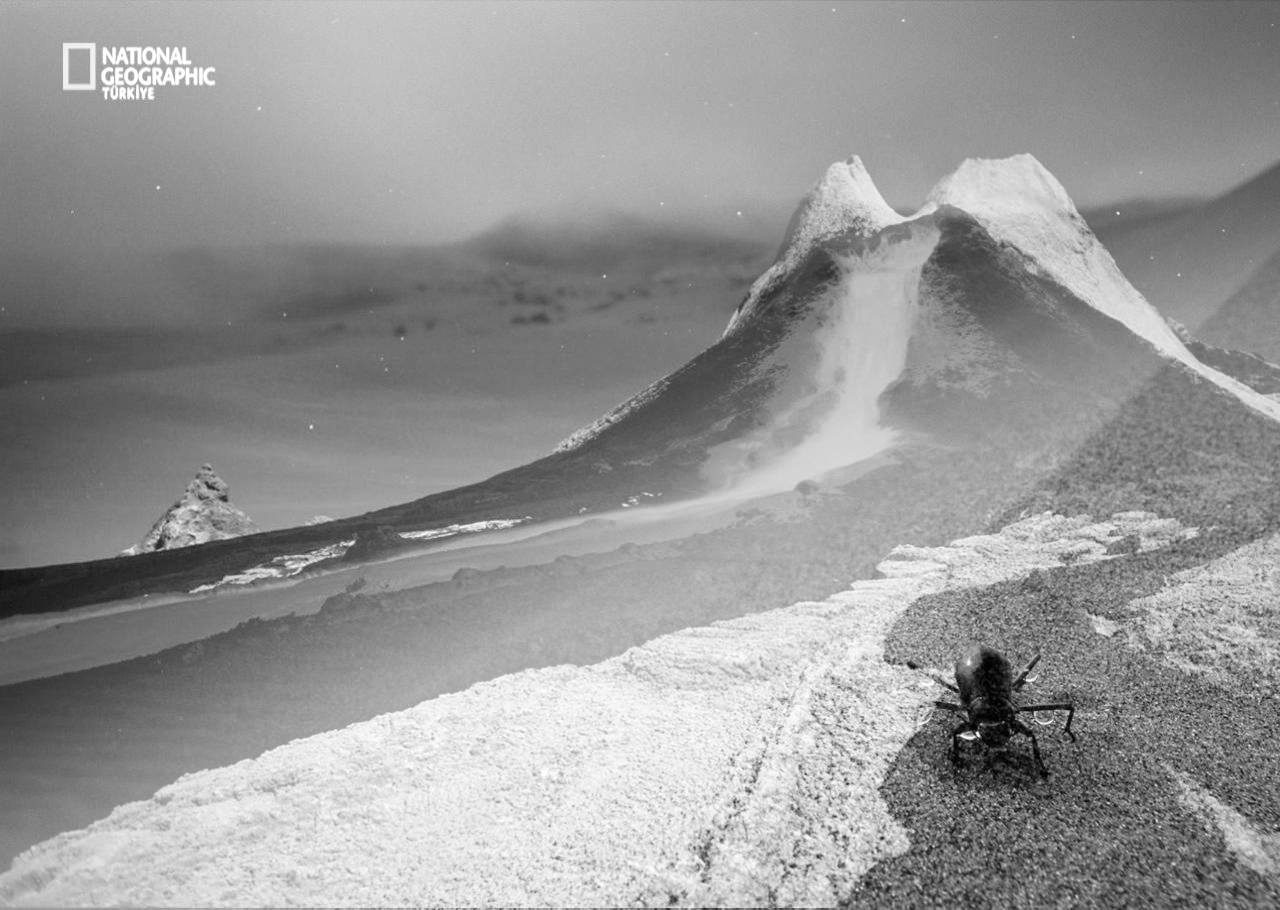
\includegraphics[width=5.5 cm]{images/sums/m y i/sscd.png}}
		\subfigure[PLIP $C_p=3.13$]{
			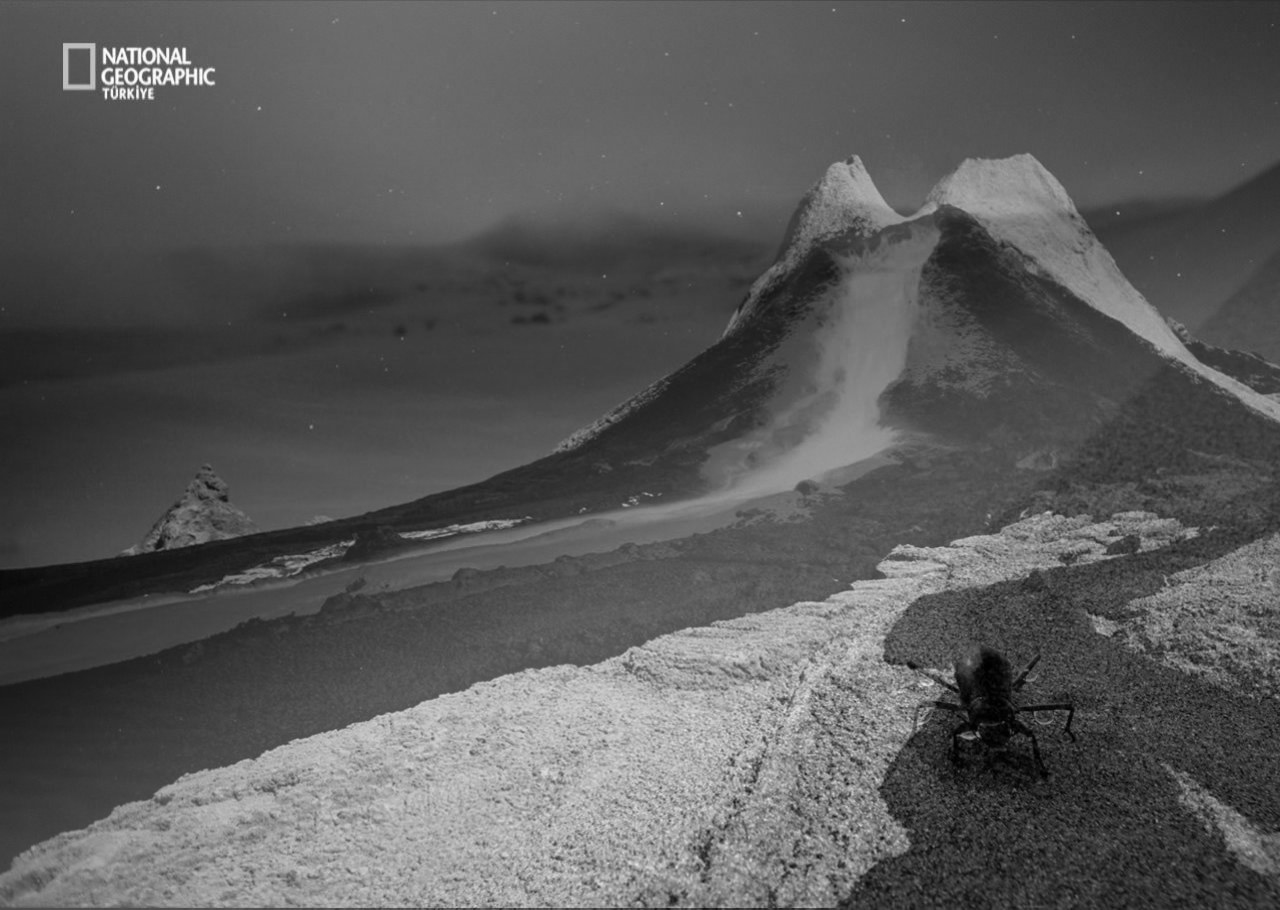
\includegraphics[width=5.5 cm]{images/sums/m y i/pscd.png}}
		\subfigure[PPSLIP $C_p=3.47$]{
			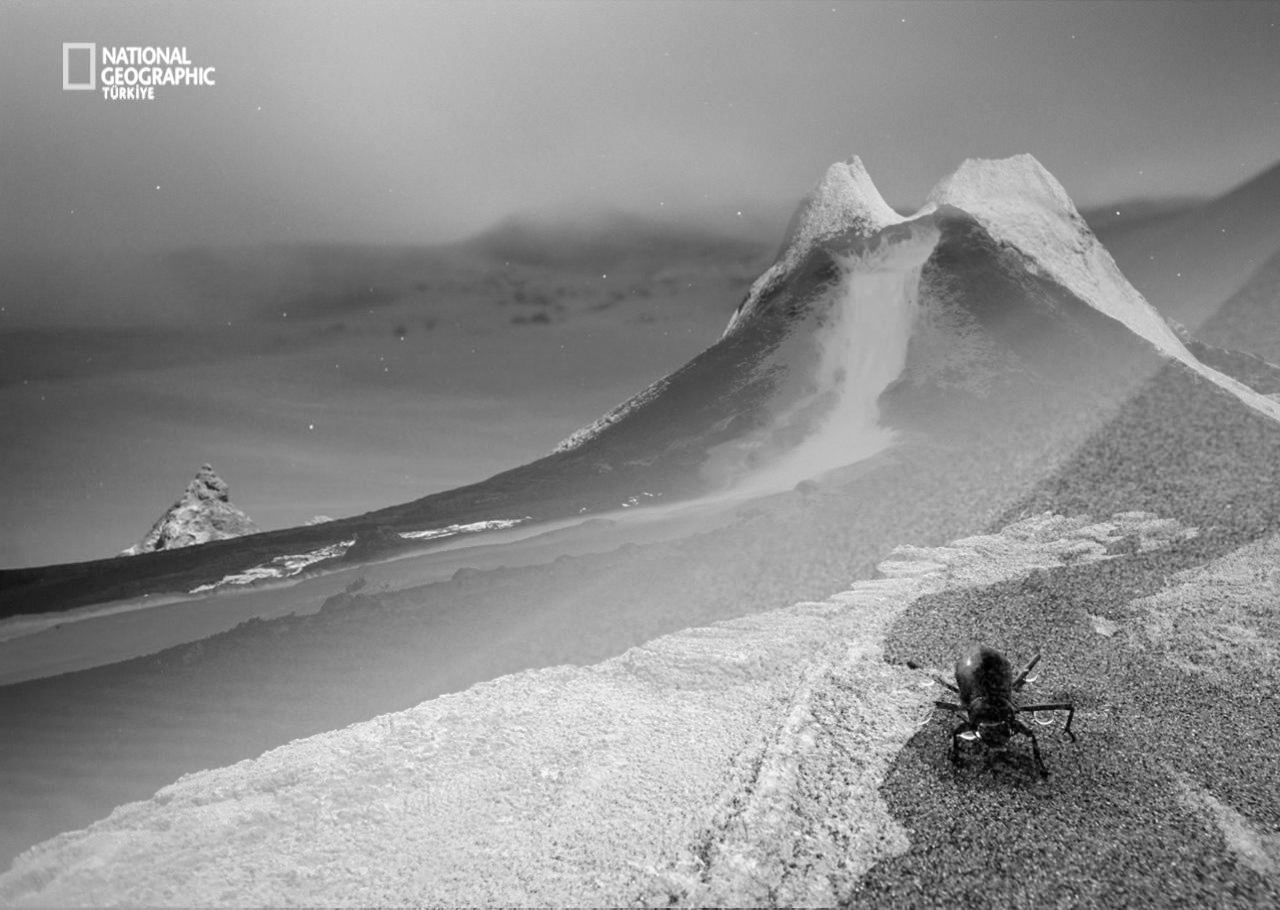
\includegraphics[width=5.5 cm]{images/sums/m y i/ppsscd.png}}
		\caption{Suma de Monta\~na e Insecto utilizando los diferentes modelos}
	\end{center}
\end{figure}

En la Figura 3.5 se muestra la suma de la imagen ``Playa'' y la imagen ''Patineta'' utilizando los diferentes modelos. En esta figura se puede apreciar que el mejor valor de contraste promedio $C_p$ es el del modelo LIP. Adem\'as se puede apreciar que las im\'agenes dada por los modelos SLIP y PSLIP son im\'agenes claras mientras que para el modelo LIP esta es m\'as oscura. Esto es l\'ogico debido a que en el modelo LIP, se invierte la escala de gris mientras que en los dos antes mencionados esto no ocurre. El modelo HLIP muestra un comportamiento balanceado, como era de esperarse debido a su simetr\'ia. Dado que el modelo LIP es que el mejor resultado arroja, en consecuencia el modelo PLIP se comporta como este, mientras que al dar, el modelo PSLIP un valor de contraste peor al del modelo lineal, es l\'ogico que este tienda a la linealidad.

Para determinar los par\'ametros de $\gamma(M)$ y $\mu(M)$ en el modelo PLIP, se aplic\'o el cambio a tonos de gris utilizando el valor de $M=256$. Luego se prob\'o la suma con diferentes valores de $\gamma(M)$ (256, 300, 1026 y 4100) y por cada uno se probaron varios valores de $\mu(M)$ para cambiar a niveles de grises. Para determinar el mejor valor de $\mu(M)$ para cada $\gamma(M)$ se utiliz\'o la m\'etrica EMEE. Luego se calcul\'o el valor de $C_p$ por cada pareja y el mejor valor se obtuvo para $\mu(M)=256$ y $\gamma(M)=256$. Para determinar el mejor valor de $\gamma(M)$ para el modelo PPSLIP se realiz\'o la operaci\'on de suma utilizando diferentes par\'ametros y se determin\'o el mejor utilizando el valor de $C_p$, el resultado fue de $\gamma(M)=4100$. 

En la Figura 3.6 se puede observar otro ejemplo de la suma. En este caso el modelo LIP arroja una imagen muy oscura, mientras que el modelo lineal ofrece una m\'as clara. M\'as claras a\'un y con mejor valor de $C_p$ son las im\'agenes obtenidas por los modelos PSLIP y SLIP. Se vuelve a apreciar el balance en el modelo HLIP, dando una imagen donde se combinan en gran medida los negros y los blancos, dando el mejor valor de $C_p$. En este caso el modelo PLIP tendi\'o a la linealidad para lograr un mejor valor de $C_p$, mientras que por su parte el modelo PPSLIP se asemej\'o al modelo PSLIP.

Con estos experimentos ya se puede ir percatando lo que te\'oricamente se esperaba: la sensibilidad del modelo PLIP hacia los niveles de gris m\'as oscuros, la sensibilidad de los modelos PSLIP y SLIP hacia los niveles de gris m\'as claros y el balance entre ambos que muestra el modelo HLIP dado su car\'acter sim\'etrico. Aqu\'i aclarar que el modelo SLIP, aunque tambi\'en es sim\'etrico, una imagen trasformada a este modelo no se expande por toda la escala de gris del modelo como si ocurre en el HLIP, a no ser que se haga esto manualmente. Tambi\'en se puede apreciar como los modelos parametrizados utilizan los par\'ametros buscando la linealidad, para, en el caso del PLIP obtener una imagen m\'as clara, y para el caso del PPSLIP obtener una imagen m\'as oscura. 

\subsubsection{Estad\'isticas}

\begin{figure}
	\begin{center}
		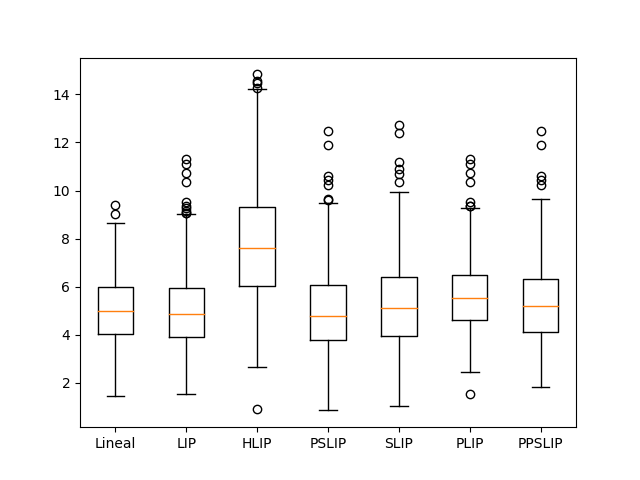
\includegraphics[width=10.0 cm]{images/graphics/sum_all.png}
		\caption{Comparaci\'on estad\'istica de los diferentes modelos para la operaci\'on suma utilizando im\'agenes naturales}
	\end{center}
\end{figure}

\begin{table}
	\begin{center}
		\begin{tabular}{|l|l|l|}
			\hline 
			Modelo & Media & Mediana\\
			\hline
			Lineal & $5.05$ & $4.98$\\
			\hline
			LIP & $5.00$ & $4.85$\\
			\hline
			HLIP & $7.73$ & $7.59$\\
			\hline
			PSLIP & $4.95$ & $4.78$\\
			\hline
			SLIP & $5.24$ & $5.08$\\
			\hline
			PLIP & $5.60$ & $5.54$\\
			\hline
			PPSLIP & $5.35$ & $5.20$\\
			\hline
		\end{tabular}
		\caption{Media y Mediana para la operaci\'on suma de los diferentes modelos utilizando im\'agenes naturales}
	\end{center}
\end{table}

En la Figura 3.7 y en la Tabla 3.1 se puede ver una comparaci\'on de la suma de dos im\'agenes utilizando los diferentes modelos. Se aprecia que los modelos lineal y LIP presentan un desempe\~no un tanto similar y el SLIP fue un tanto superior a ambos. Estos nos habla que en el conjunto de datos utilizado en los experimentos, las im\'agenes presentan un balance entre tonalidades oscuras y claras, aunque con una mayor presencia de tonalidades oscuras pero sin que exista una diferencia considerable. Por esto el mejor resultado se obtiene para el modelo HLIP, que gracias a su simetr\'ia permite obtener im\'agenes de mayor contraste. Este modelo muestra un valor de $Cp$ promedio de $7.73$ y para el el $50\%$ de los datos se obtiene un valor superior o igual a $7.59$. Ob\'ervese que los modelos parametrizados dan mejores resultados que el lineal y sus modelos no parametrizados correspondientes, por lo que se se puede concluir que la parametrizaci\'on result\'o \'util.  

\subsection{Detecci\'on de Bordes}

En esta secci\'on se muestra una comparaci\'on entre los diferentes modelos utilizando el filtro de Scharr para la detecci\'on de bordes. Para la realizaci\'on de estos experimentos se pueden utilizar las funciones descritas en la secci\'on \textbf{Detalles de Implementaci\'on} o se puede hacer el proceso descrito manualmente. 

\subsubsection{Ejemplos}

En estos experimentos se utilizaron las im\'agenes: C\'amara y T\'orax 1 que se muestran en la Figura 3.8. La primera es una imagen natural y la segunda una imagen m\'edica de una radiograf\'ia. Los experimentos realizados se pueden ver en la Figura 3.9 y Figura 3.10 respectivamente.

\begin{figure}
	\begin{center}
		\subfigure[C\'amara]{
			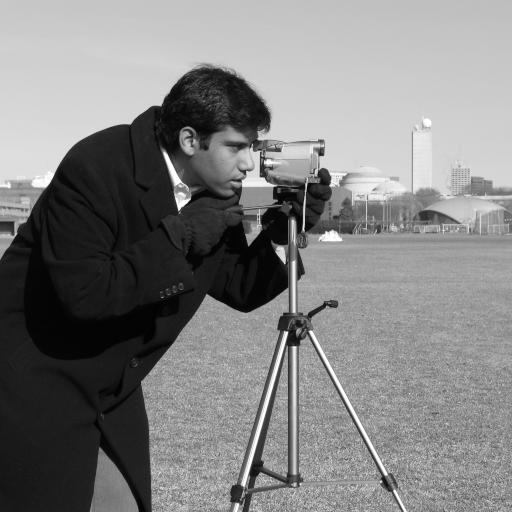
\includegraphics[width=5.0 cm]{images/originals/camera.jpg}}
		\subfigure[T\'orax 1]{
			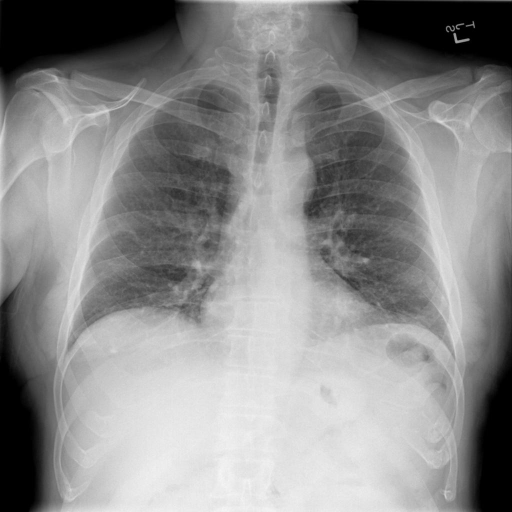
\includegraphics[width=5.0 cm]{images/originals/torax.png}}
		\caption{Im\'agenes para los experimentos de detecci\'on de bordes}
	\end{center}
\end{figure}

\begin{figure}
	\begin{center}
		\subfigure[Lineal $C_p=4.69$]{
			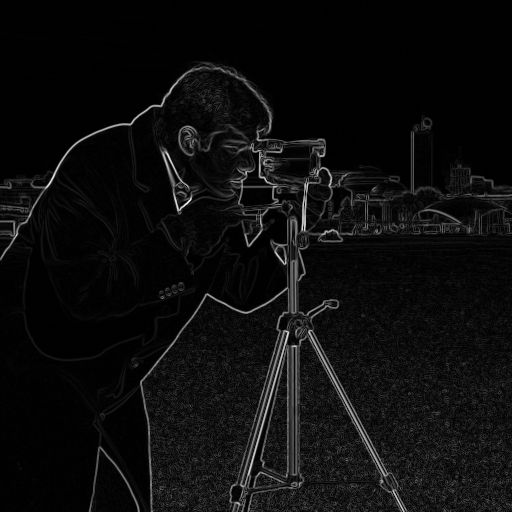
\includegraphics[width=4.0 cm]{images/scharr/camera/sla.png}}
		\subfigure[LIP $C_p=7.43$]{
			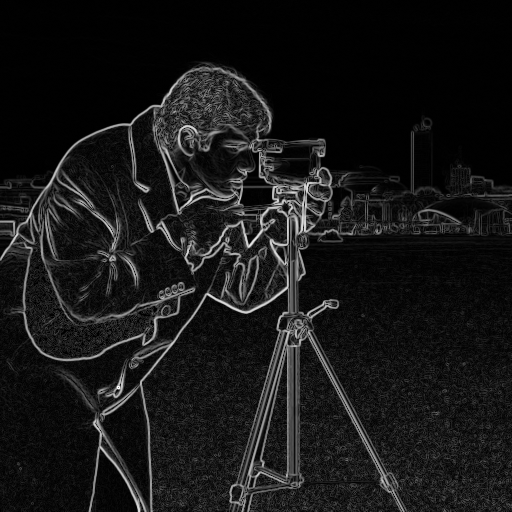
\includegraphics[width=4.0 cm]{images/scharr/camera/sja.png}}
		\subfigure[HLIP $C_p=8.05$]{
			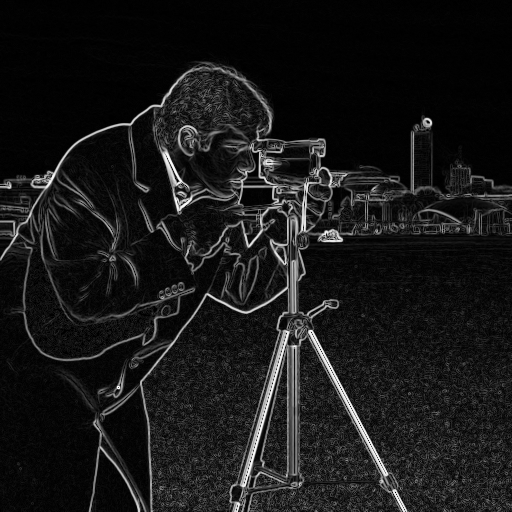
\includegraphics[width=4.0 cm]{images/scharr/camera/sha.png}}
		\subfigure[PSLIP $C_p=9.41$]{
			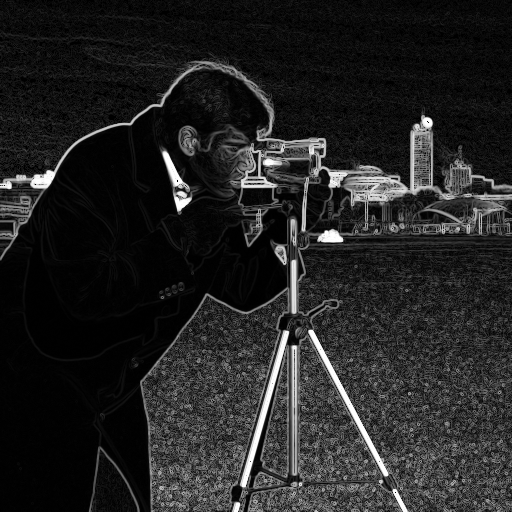
\includegraphics[width=4.0 cm]{images/scharr/camera/spsa.png}}
		\subfigure[SLIP $C_p=6.26$]{
			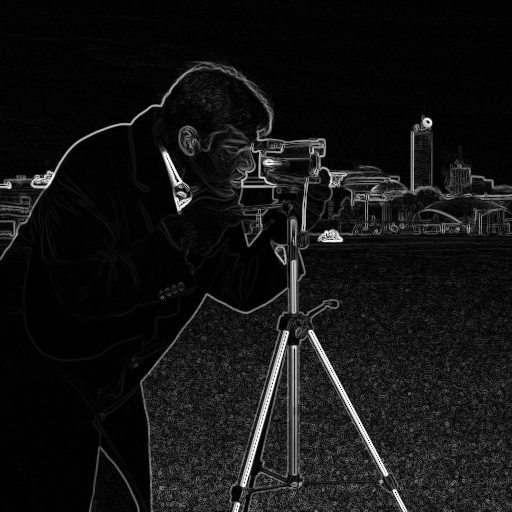
\includegraphics[width=4.0 cm]{images/scharr/camera/ssa.png}}
		\subfigure[PLIP $C_p=7.43$]{
			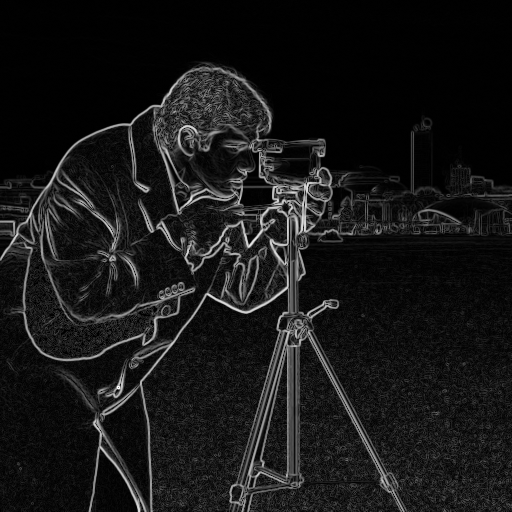
\includegraphics[width=4.0 cm]{images/scharr/camera/spa.png}}
		\subfigure[PPSLIP $C_p=9.41$]{
			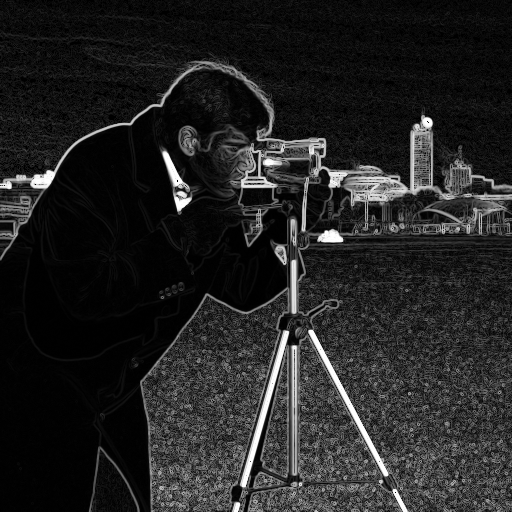
\includegraphics[width=4.0 cm]{images/scharr/camera/sppsa.png}}
		\caption{Filtro de Scharr aplicado a la imagen C\'amara con los diferentes modelos}
	\end{center}
\end{figure}

\begin{figure}
	\begin{center}
		\subfigure[Lineal $C_p=2.89$]{
			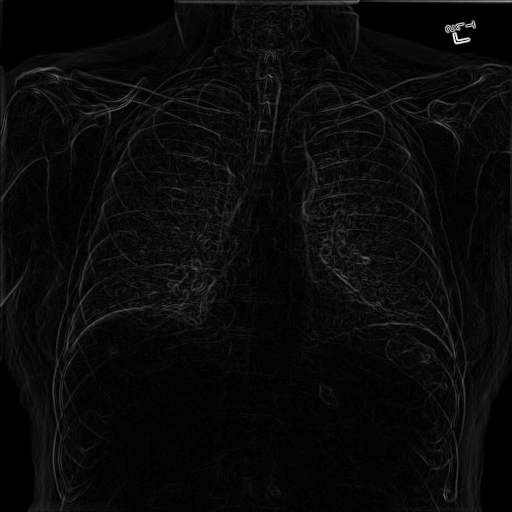
\includegraphics[width=4.0 cm]{images/scharr/torax/slb.png}}
		\subfigure[LIP $C_p=3.66$]{
			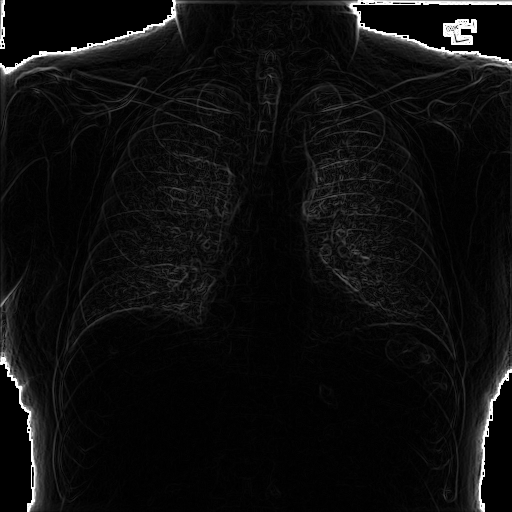
\includegraphics[width=4.0 cm]{images/scharr/torax/sjb.png}}
		\subfigure[HLIP $C_p=4.40$]{
			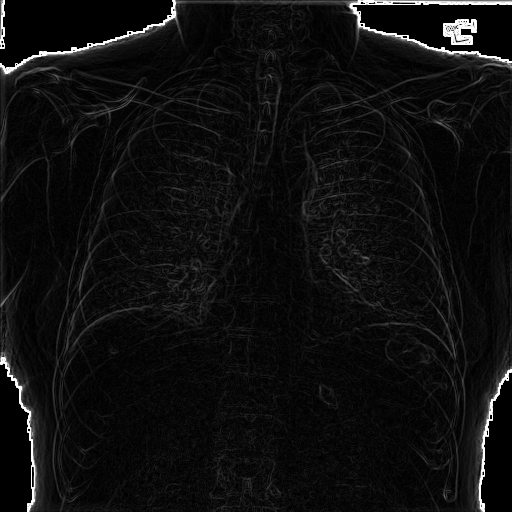
\includegraphics[width=4.0 cm]{images/scharr/torax/shb.png}}
		\subfigure[PSLIP $C_p=9.73$]{
			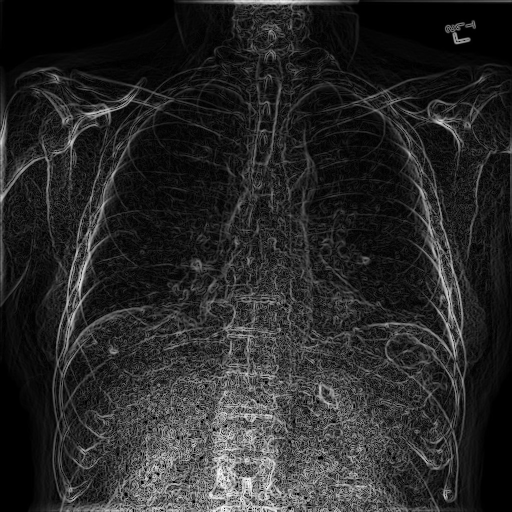
\includegraphics[width=4.0 cm]{images/scharr/torax/spsb.png}}
		\subfigure[SLIP $C_p=6.85$]{
			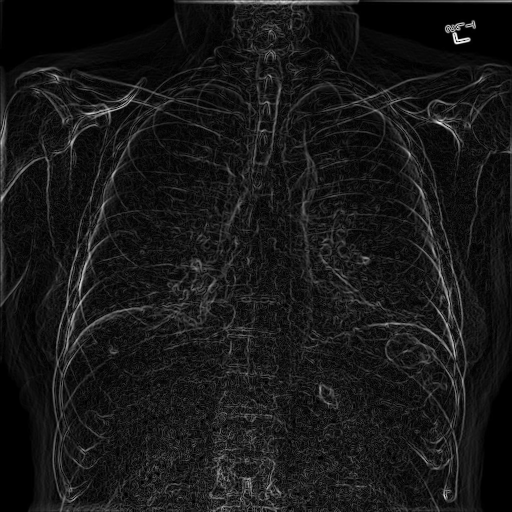
\includegraphics[width=4.0 cm]{images/scharr/torax/ssb.png}}
		\subfigure[PLIP $C_p=3.66$]{
			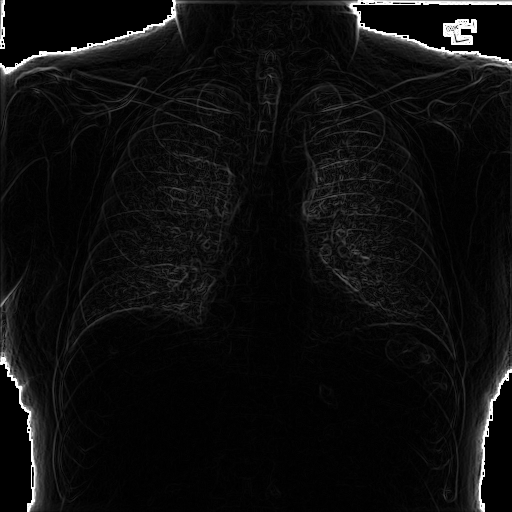
\includegraphics[width=4.0 cm]{images/scharr/torax/spb.png}}
		\subfigure[PPSLIP $C_p=9.73$]{
			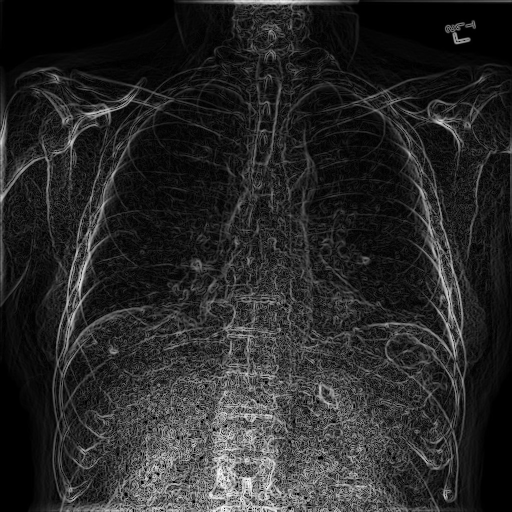
\includegraphics[width=4.0 cm]{images/scharr/torax/sppsb.png}}
		\caption{Filtro de Scharr aplicado a la imagen T\'orax 1 con los diferentes modelos}
	\end{center}
\end{figure} 

Como se puede ver en la Figura 3.9 el modelo lineal se queda bastante rezagado con respecto a los modelos no lineales en cuanto al contraste promedio $C_p$. Esto adem\'as lo evidencia que el modelo PLIP arroj\'o un resultado similar al modelo LIP. Otro detalle es que el modelo LIP detect\'o mejor los bordes en las tonalidades m\'as oscuras, mientras que el SLIP hizo lo propio para las tonalidades m\'as claras. Clara evidencia esto de a que niveles de gris son m\'as sensibles estos dos modelos. El modelo HLIP por su parte dio un resultado m\'as balanceado arrojando un valor de $C_p$ superior a los anteriores. Para este caso el mejor resultado se obtuvo utilizando el modelo PSLIP, lo cual se puede comprobar visualmente y mediante el valor de $C_p$, esto gracias a la gran sensibilidad de este modelo a las tonalidades m\'as claras, lo cual era de esperarse al ver la curva de dicho isomorfismo. Dada que este fue el mejor resultado, por ende el modelo PPSLIP coincide con este. Aunque el PSLIP da muy buenos resultados se puede apreciar que para las tonalidades oscuras es superado por el LIP y el HLIP, una soluci\'on a esto pudiera ser invertir la escala de grises tal como se hace en el modelo LIP, aunque se perder\'ia la gran sensibilidad a tonalidades claras. Otra soluci\'on para mantener la sensibilidad hacia ambas tonalidades ser\'ia hacer este modelo sim\'etrico. Adem\'as se debe tener cuidado ya que su alta sensibilidad lo hace tambi\'en muy sensible al ruido.

En este experimento los par\'ametros a estimar fueron $\lambda(M)$ para PLIP y PPSLIP, adem\'as de $\mu(M)$ en el caso de PLIP. La selecci\'on de estos par\'ametros se hizo de una forma similar a la explicada para la suma, lo que obviamente aplicada a la funci\'on del isomorfismo.

Un uso muy pr\'actico de los filtros para la detecci\'on de bordes es en im\'agenes m\'edicas. Como se dijo anteriormente un ejemplo de estos se puede apreciar en la Figura 3.10 utilizando los diferentes modelos. En este ejemplo se puede apreciar visualmente como todos los modelos no lineales superan al modelo lineal, lo cual es confirmado por el valor de $C_p$. Al ser una imagen donde predominan las tonalidades claras es l\'ogico que el modelo LIP arroje los peores resultados, seguido del modelo HLIP. El SLIP arroja un muy buen resultado, pero es superado en gran medida por el modelo PSLIP (y por ende el PPSLIP), dando una imagen muy detallada y de muy buena calidad. El valor de $C_p$ confirma esta apreciaci\'on visual.

\subsubsection{Estad\'isticas}

\begin{figure}
	\begin{center}
		\includegraphics[width=10.0 cm]{images/graphics/natural/ed/ed_all.png}
		\caption{Comparaci\'on estad\'istica en cuanto al valor de $C_p$ utilizando los diferentes modelos para la detecci\'on de bordes en im\'agenes naturales}
	\end{center}
\end{figure}

\begin{table}
	\begin{center}
		\begin{tabular}{|l|l|l|}
			\hline 
			Modelo & Media & Mediana\\
			\hline
			Lineal & $5.02$ & $4.75$\\
			\hline
			LIP & $11.55$ & $10.82$\\
			\hline
			HLIP & $12.81$ & $12.36$\\
			\hline
			PSLIP & $11.57$ & $11.38$\\
			\hline
			SLIP & $9.30$ & $8.91$\\
			\hline
			PLIP & $11.59$ & $10.82$\\
			\hline
			PPSLIP & $11.65$ & $11.47$\\
			\hline
		\end{tabular}
		\caption{Media y mediana del valor de $C_p$ para la detecci\'on de bordes utilizando los diferentes modelos en im\'agenes naturales}
	\end{center}
\end{table}

En la Figura 3.11 y la Tabla 3.2 se ofrece una comparativa utilizando los diferentes modelos para la detecci\'on de bordes en im\'agenes naturales. Se aprecia como el modelo lineal queda muy rezagado con respecto a los modelos no lineales. En estas im\'agenes el modelo LIP y el PSLIP muestran buenos resultados, aunque siendo un poco superior el PSLIP. Si bien la parametrizaci\'on de los modelos muestra una mejora con respecto a los no parametrizados esta no es muy significativa. El mejor resultado lo ofrece el modelo HLIP que como se vi\'o en el ejemplo presentado es sensible tanto a las tonalidades claras como a las oscuras permitiendo captar de gran manera los bordes en ambos casos. Este modelo present\'o un valor de $C_p$ promedio de $12.81$ y para el $50\%$ de los casos se obtuvo un valor igual o superior a $12.36$. 

\begin{figure}
	\begin{center}
		\includegraphics[width=10.0 cm]{images/graphics/torax/ed/ed_all.png}
		\caption{Comparaci\'on estad\'istica en cuanto al valor de $C_p$ utilizando los diferentes modelos para la detecci\'on de bordes en im\'agenes de radiograf\'ias de t\'orax}
	\end{center}
\end{figure}

\begin{table}
	\begin{center}
		\begin{tabular}{|l|l|l|}
			\hline 
			Modelo & Media & Mediana\\
			\hline
			Lineal & $0.96$ & $0.89$\\
			\hline
			LIP & $3.48$ & $3.38$\\
			\hline
			HLIP & $3.69$ & $3.85$\\
			\hline
			PSLIP & $5.55$ & $5.38$\\
			\hline
			SLIP & $3.11$ & $3.09$\\
			\hline
			PLIP & $3.68$ & $3.60$\\
			\hline
			PPSLIP & $5.64$ & $5.41$\\
			\hline
		\end{tabular}
		\caption{Media y mediana del valor de $C_p$ para la detecci\'on de bordes utilizando los diferentes modelos en im\'agenes de radiograf\'ias de t\'orax}
	\end{center}
\end{table}

En la Figura 3.12 y la Tabla 3.3 se aprecia la misma comparativa pero utilizando las im\'agenes m\'edicas de radiograf\'ias de t\'orax. Se aprecia igual que el modelo lineal queda muy por debajo de los modelos no lineales. Los modelos LIP, HLIP y SLIP dan buenos resultados, pero son ampliamente superados por el modelo PSLIP, y adem\'as la parametrizaci\'on hace que el gran vencedor sea el modelo PPSLIP, dando un valor de $C_p$ promedio de $5.64$ y un valor igual o superior a $5.41$ para el $50\%$  de los casos. Esto pasa ya que las im\'agenes de radiograf\'ias, por lo general, son im\'agenes con un fondo oscuro y la informaci\'on la portan las tonalidades blancas a las cuales el modelo PSLIP es altamente sensible como se vio en el ejemplo mostrado. Luego adem\'as la parametrizaci\'on arroja a\'un mejores resultados. 

\subsection{Unsharp Masking}

Los pr\'oximos experimentos que se presentan a continuaci\'on son la aplicaci\'on del algoritmo de \textit{Unsharp Masking} utilizando los diferentes modelos. Para la realizaci\'on de los mismos, al igual que en los casos anteriores, se pueden utilizar las funciones implementadas para este cometido y que fueron descritas en la secci\'on \textbf{Detalles de implementaci\'on} o hacerlo manualmente siguiendo el procedimiento descrito.

\subsubsection{Ejemplos}

Las im\'agenes utilizadas en estos ejemplos son las mismas ya usadas anteriormente: C\'amara y T\'orax 1. Los resultados de estos experimentos se pueden apreciar en las Figura 3.13 y Figura 3.14 respectivamente.

\begin{figure}
	\begin{center}
		\subfigure[Original $C_p=5.00$]{
			\includegraphics[width=4.0 cm]{images/unsharp_masking/camera/camera.png}}
		\subfigure[Lineal $C_p=4.13$]{
			\includegraphics[width=4.0 cm]{images/unsharp_masking/camera/la_sla.png}}
		\subfigure[LIP $C_p=5.14$]{
			\includegraphics[width=4.0 cm]{images/unsharp_masking/camera/ja_sja.png}}
		\subfigure[HLIP+ $C_p=5.66$]{
			\includegraphics[width=4.0 cm]{images/unsharp_masking/camera/ha_sha+.png}}
		\subfigure[HLIP- $C_p=5.73$]{
			\includegraphics[width=4.0 cm]{images/unsharp_masking/camera/ha_sha-.png}}
		\subfigure[PSLIP $C_p=4.84$]{
			\includegraphics[width=4.0 cm]{images/unsharp_masking/camera/psa_spsa.png}}
		\subfigure[SLIP $C_p=5.16$]{
			\includegraphics[width=4.0 cm]{images/unsharp_masking/camera/sa_ssa.png}}
		\subfigure[PLIP $C_p=5.14$]{
			\includegraphics[width=4.0 cm]{images/unsharp_masking/camera/pa_spa.png}}
		\subfigure[PPSLIP $C_p=5.80$]{
			\includegraphics[width=4.0 cm]{images/unsharp_masking/camera/ppsa_sppsa.png}}
		\caption{Unsharp masking aplicado a la imagen C\'amara con los diferentes modelos}
	\end{center}
\end{figure}

\begin{figure}
	\begin{center}
		\subfigure[Original $C_p=2.26$]{
			\includegraphics[width=4.0 cm]{images/unsharp_masking/torax/CXR7_IM-2263-1001.png}}
		\subfigure[Lineal $C_p=2.60$]{
			\includegraphics[width=4.0 cm]{images/unsharp_masking/torax/lb_slb.png}}
		\subfigure[LIP $C_p=2.53$]{
			\includegraphics[width=4.0 cm]{images/unsharp_masking/torax/jb_sjb.png}}
		\subfigure[HLIP+ $C_p=3.46$]{
			\includegraphics[width=4.0 cm]{images/unsharp_masking/torax/hb_shb+.png}}
		\subfigure[HLIP- $C_p=2.62$]{
			\includegraphics[width=4.0 cm]{images/unsharp_masking/torax/hb_shb-.png}}
		\subfigure[PSLIP $C_p=2.52$]{
			\includegraphics[width=4.0 cm]{images/unsharp_masking/torax/psb_spsb.png}}
		\subfigure[SLIP $C_p=2.59$]{
			\includegraphics[width=4.0 cm]{images/unsharp_masking/torax/sb_ssb.png}}
		\subfigure[PLIP $C_p=2.53$]{
			\includegraphics[width=4.0 cm]{images/unsharp_masking/torax/pb_spb.png}}
		\subfigure[PPSLIP $C_p=4.97$]{
			\includegraphics[width=4.0 cm]{images/unsharp_masking/torax/ppsb_sppsb.png}}
		\caption{Unsharp masking aplicado a la imagen T\'orax 1 con los diferentes modelos}
	\end{center}
\end{figure}

En la Figura 3.13 se puede apreciar como este algoritmo para el caso lineal de una imagen incluso peor a la imagen original pues esta es muy oscura y los bordes no se aprecian muy bien definidos, lo cual tambi\'en lo confirma el valor de $C_p$. El modelo LIP da una mejor soluci\'on. Aprovech\'andose el car\'acter sim\'etrico del modelo HLIP se analizaron dos variantes de fusi\'on: la suma y la resta. Para este ejemplo se puede comprobar visualmente que la mejor imagen obtenida fue la resultante de la fusi\'on mediante la resta, lo cual tambi\'en es confirmado por el valor de $C_p$. 

El modelo PSLIP tampoco ofrece un mejor resultado, esto debido a que no se logra una buena fusi\'on entre la imagen original y la imagen de bordes, algo similar a lo que ocurri\'o en en el primer experimento de suma de im\'agenes presentado. El modelo SLIP tambi\'en da un buen resultado, con un valor de $C_p$ muy parecido al del modelo LIP. El modelo PLIP se asemej\'o a un comportamiento logar\'itmico como era de esperarse dados los resultados del modelo lineal y del LIP. Tambi\'en se puede apreciar como el modelo PPSLIP resuelve el problema del modelo PSLIP, arrojando una imagen de mayor calidad, siendo esta la de mejor valor de $C_p$. V\'alido se\~nalar que esta \'ultima resalta mucho los bordes por lo que quiz\'as ser\'ia mejor utilizar otro modelo o utilizar par\'ametros que den una imagen m\'as suave seg\'un la situaci\'on.

Aqu\'i tambi\'en es bueno aclarar que para los modelos parametrizados se utiliz\'o como par\'ametro para la funci\'on del isomorfismo el par\'ametro que di\'o el mejor resultado en la detecci\'on de bordes para cada modelo. Dado esto, entonces, lo que se hizo fue buscar los mejores par\'ametros que dieran el mejor resultado para la fusi\'on.

En la Figura 3.14 si bien todos los modelos resaltan en alguna medida los bordes y mejoran el valor de contraste promedio con respecto a la imagen original, los resultados no se diferencian mucho unos de otros, salvo los casos del modelo HLIP con fusi\'on por suma y del PPSLIP. Este \'ultimo arroja una imagen mucho m\'as detallada y por ende de mayor calidad que el resto de los modelos, algo que se puede comprobar tanto visualmente como por el valor de $C_p$. Esto confirma una vez m\'as la eficacia y utilidad del modelo propuesto.

\subsubsection{Estad\'isticas}

\begin{figure}
	\begin{center}
		\includegraphics[width=10.0 cm]{images/graphics/natural/unsharp_masking/um_all.png}
		\caption{Comparaci\'on estad\'istica en cuanto al valor de $C_p$ utilizando los diferentes modelos para el algoritmo \textit{unsharp masking} en im\'agenes naturales}
	\end{center}
\end{figure}

\begin{table}
	\begin{center}
		\begin{tabular}{|l|l|l|}
			\hline 
			Modelo & Media & Mediana\\
			\hline
			Original & $7.63$ & $7.07$\\
			\hline
			Lineal & $6.04$ & $5.66$\\
			\hline
			LIP & $7.24$ & $6.81$\\
			\hline
			HLIP+ & $9.67$ & $9.07$\\
			\hline
			HLIP- & $8.23$ & $7.52$\\
			\hline
			PSLIP & $7.10$ & $6.73$\\
			\hline
			SLIP & $7.65$ & $7.24$\\
			\hline
			PLIP & $7.95$ & $7.72$\\
			\hline
			PPSLIP & $7.99$ & $7.84$\\
			\hline
		\end{tabular}
		\caption{Media y mediana del valor de $C_p$ para el algoritmo \textit{unsharp masking} utilizando los diferentes modelos en im\'agenes naturales}
	\end{center}
\end{table}

En la Figura 3.15 y la Tabla 3.4 se puede apreciar una comparaci\'on de este algoritmo en im\'agenes naturales. Los mejores resultados se obtuvieron para el modelo HLIP, tanto para la fusi\'on por suma como para la fusi\'on por resta, aunque siendo la suma un tanto superior. Esto se pod\'ia esperar ya que el modelo HLIP fue el mejor modelo tanto para la detecci\'on de bordes en im\'agenes naturales como para la suma de im\'agenes, las dos operaciones que se hacen en este algoritmo. Utilizando el modelo HLIP con fusi\'on por suma se obtuvo un valor de $C_p$ promedio de $9.67$ y un valor igual o superior a $9.07$ para el $50\%$ de los casos. Tambi\'en se aprecia como los modelos parametrizados superan tanto al lineal como a sus respectivos modelos no parametrizados.

\begin{figure}
	\begin{center}
		\includegraphics[width=10.0 cm]{images/graphics/torax/unsharp_masking/um_all.png}
		\caption{Comparaci\'on estad\'istica en cuanto al valor de $C_p$ utilizando los diferentes modelos para el algoritmo \textit{unsharp masking} en im\'agenes de radiograf\'ias de t\'orax}
	\end{center}
\end{figure}

\begin{table}
	\begin{center}
		\begin{tabular}{|l|l|l|}
			\hline 
			Modelo & Media & Mediana\\
			\hline
			Original & $1.64$ & $1.57$\\
			\hline
			Lineal & $1.49$ & $1.42$\\
			\hline
			LIP & $1.88$ & $1.78$\\
			\hline
			HLIP+ & $2.71$ & $2.78$\\
			\hline
			HLIP- & $1.91$ & $1.82$\\
			\hline
			PSLIP & $1.84$ & $1.78$\\
			\hline
			SLIP & $1.87$ & $1.80$\\
			\hline
			PLIP & $2.21$ & $2.27$\\
			\hline
			PPSLIP & $3.00$ & $2.94$\\
			\hline
		\end{tabular}
		\caption{Media y mediana del valor de $C_p$ para el algoritmo \textit{unsharp masking} utilizando los diferentes modelos en im\'agenes de radiograf\'ias de t\'orax}
	\end{center}
\end{table}

En la Figura 3.16 y la Tabla 3.5 se puede apreciar una comparaci\'on de este algoritmo en im\'agenes de radiograf\'ias de t\'orax. Aqu\'i se aprecia que aunque el modelo HLIP  utilizando fusi\'on por suma, sigue ofreciendo resultados destacables; el mejor desempe\~no corresponde al modelo PPSLIP propuesto el cual aprovecha la sensibilidad del modelo PSLIP para detectar bordes, la cual mejora incluso con la ayuda de la parametrizaci\'on, y adem\'as utiliza esta para realizar la suma resolviendo el problema del d\'ebil desempe\~no que si presenta el modelo PSLIP para esta operaci\'on. Para el modelo PPSLIP se obtiene un valor de $C_p$ promedio de $3.00$, dando un valor igual o superior a $2.94$ para el $50\%$ de los casos.

\subsection{Transformaci\'on af\'in}

A continuaci\'on se presentan los experimentos basados en la modificaci\'on del histograma. Espec\'ificamente se analizar\'a la ecualizaci\'on del histograma que  que ``extiende los valores de intensidad más frecuentes'' y ya viene implementada el m\'odulo \verb|skimage.exposure|~\cite{histogram_equalization}. Aunque si bien la ecualización del histograma tiene la ventaja de que no requiere parámetros, a veces produce imágenes de aspecto poco natural. Los otros algoritmos analizados ser\'a el de transformaci\'on af\'in utilizando los modelos HLIP y SLIP. Para el caso del modelo SLIP antes de aplicar la transformaci\'on af\'in primero se extiende la imagen por todo el rango de valores $(-M,M)$, utilizando la transformaci\'on lineal $2f-M\cdot\frac{255}{256}$ donde $f$ es una imagen. Esta transformaci\'on se hizo para aprovechar todo el rango de valores del modelo SLIP y obtener mejores resultados pero no es algo inherente al modelo. Esta es una de las ventajas que tiene usar los modelos definidos desde un punto de vista de matem\'atico. 

\subsubsection{Ejemplos}

Las im\'agenes utilizadas en los ejemplos que se presentan son im\'agenes de bajo contraste: Luna y T\'orax 2. Los experimentos sobre estas im\'agenes se pueden observar en las Figura 3.17 y Figura 3.18 respectivamente.

\begin{figure}
	\begin{center}
		\subfigure[Original $C_p=1.30$]{
			\includegraphics[width=4.3 cm]{images/he/moon/imgs/moon.png}}
		\subfigure[Original Histograma]{
			\includegraphics[width=6.0 cm]{images/he/moon/hists/oa_hist.png}}
		\subfigure[Ecualizada $C_p=10.86$]{
			\includegraphics[width=4.3 cm]{images/he/moon/imgs/limg_eq_a.png}}
		\subfigure[Ecualizada Histograma]{
			\includegraphics[width=6.0 cm]{images/he/moon/hists/leqa_hist.png}}
		\subfigure[Transformaci\'on HLIP $C_p=5.35$]{
			\includegraphics[width=4.33 cm]{images/he/moon/imgs/himg_eq_a.png}}
		\subfigure[Transformaci\'on HLIP Histograma]{
			\includegraphics[width=6.0 cm]{images/he/moon/hists/hata_hist.png}}
		\subfigure[Transformaci\'on SLIP $C_p=5.07$]{
			\includegraphics[width=4.3 cm]{images/he/moon/imgs/simg_eq_a.png}}
		\subfigure[Transformaci\'on SLIP Histograma]{
			\includegraphics[width=6.0 cm]{images/he/moon/hists/sata_hist.png}}
		\caption{Diferentes t\'ecnicas de modificaci\'on del histograma de la imagen Luna}
	\end{center}
\end{figure}

\begin{figure}
	\begin{center}
		\subfigure[Original $C_p=1.05$]{
			\includegraphics[width=5.0 cm]{images/he/torax/imgs/torax.png}}
		\subfigure[Original Histograma]{
			\includegraphics[width=5.5 cm]{images/he/torax/hists/ob_hist.png}}
		\subfigure[Ecualizada $C_p=2.82$]{
			\includegraphics[width=5.0 cm]{images/he/torax/imgs/limg_eq_b.png}}
		\subfigure[Ecualizada Histograma]{
			\includegraphics[width=5.5 cm]{images/he/torax/hists/leqb_hist.png}}
		\subfigure[Transformaci\'on HLIP $C_p=2.36$]{
			\includegraphics[width=5.0 cm]{images/he/torax/imgs/himg_eq_b.png}}
		\subfigure[Transformaci\'on HLIP Histograma]{
			\includegraphics[width=5.5 cm]{images/he/torax/hists/hatb_hist.png}}
		\subfigure[Transformaci\'on SLIP $C_p=2.19$]{
			\includegraphics[width=5.0 cm]{images/he/torax/imgs/simg_eq_b.png}}
		\subfigure[Transformaci\'on SLIP Histograma]{
			\includegraphics[width=5.5 cm]{images/he/torax/hists/satb_hist.png}}
		\caption{Diferentes t\'ecnicas de modificaci\'on del histograma de la imagen T\'orax 2}
	\end{center}
\end{figure}

En la Figura 3.17 se puede apreciar de forma visual como la imagen Luna es una imagen con muy poco contraste. Su histograma y el valor de $C_p$ confirman esta apreciaci\'on. Luego se ve como aplicando una ecualizaci\'on del histograma la imagen mejora su contraste, pero quiz\'as se pueda considerar como una imagen poco natural, aunque esto ya es una cuesti\'on subjetiva. Aqu\'i es bueno recalcar que a pesar de que el valor de contraste promedio ($C_p$) en los experimentos realizados ha mostrado resultados consecuentes con la calidad de la imagen, esto no quiere decir que la calidad de una imagen dependa exclusivamente de su contraste, de hecho no lo hace. Para determinar la calidad de una imagen se pueden utilizar otras medidas objetivas pero al final lo m\'as importante es la calidad que pueda percibir un usuario al mirar la imagen, lo cual es una medida subjetiva. Bajo este criterio es posible que se prefieran transformaciones m\'as suaves como las que arrojan las transformaciones afines en los modelos HLIP y SLIP. Para ambos modelos se obtiene un buen valor de contraste y la imagen obtenida se percibe bastante natural.

En la Figura 3.18 observamos que la imagen del t\'orax captada por el equipo que la tomo tuvo igual un muy bajo contraste; y como los diferentes algoritmos dan resultados que mejoran tanto la calidad visual percibida como el valor de contraste promedio. Esto tambi\'en se ve reflejado en como se expanden los valores de intensidad por el histograma.

Al fijarse en los histogramas de ambas figuras se puede comprobar como la ecualizaci\'on del histograma es la transformaci\'on m\'as fuerte, la transformaci\'on af\'in utilizando el modelo HLIP  es muy parecida a la transformaci\'on af\'in utilizando el modelo SLIP, aunque la del HLIP es un poco m\'as fuerte. Esto adem\'as es confirmado por el valor de $C_p$ en ambos casos.

\subsubsection{Estad\'isticas}

\begin{figure}
	\begin{center}
		\includegraphics[width=10.0 cm]{images/graphics/natural/affine_transform/eq_all.png}
		\caption{Comparaci\'on estad\'istica en cuanto al valor de $C_p$ utilizando los diferentes algoritmos para la modificaci\'on del histograma en im\'agenes naturales}
	\end{center}
\end{figure}

\begin{table}
	\begin{center}
		\begin{tabular}{|l|l|l|}
			\hline 
			Modelo & Media & Mediana\\
			\hline
			Original & $7.63$ & $7.07$\\
			\hline
			Ecualizaci\'on & $10.75$ & $9.29$\\
			\hline
			TA HLIP & $9.20$ & $9.20$\\
			\hline
			TA SLIP & $9.11$ & $9.11$\\
			\hline
		\end{tabular}
		\caption{Media y mediana del valor de $C_p$ para la modificaci\'on del histograma utilizando los diferentes algoritmos en im\'agenes naturales}
	\end{center}
\end{table}

\begin{figure}
	\begin{center}
		\includegraphics[width=10.0 cm]{images/graphics/torax/affine_transform/eq_all.png}
		\caption{Comparaci\'on estad\'istica en cuanto al valor de $C_p$ utilizando los diferentes algoritmos para la modificaci\'on del histograma en im\'agenes de radiograf\'ia de t\'orax}
	\end{center}
\end{figure}

\begin{table}
	\begin{center}
		\begin{tabular}{|l|l|l|}
			\hline 
			Modelo & Media & Mediana\\
			\hline
			Original & $1.64$ & $1.57$\\
			\hline
			Ecualizaci\'on & $2.32$ & $2.24$\\
			\hline
			TA HLIP & $2.01$ & $1.89$\\
			\hline
			TA SLIP & $1.98$ & $1.86$\\
			\hline
		\end{tabular}
		\caption{Media y mediana del valor de $C_p$ para la modificaci\'on del histograma utilizando los diferentes algoritmos en im\'agenes de radiograf\'ias de t\'orax}
	\end{center}
\end{table}

En los experimentos realizados cuyos resultados se muestran en la Figura 3.19 y la Tabla 3.6 para el caso de las im\'agenes naturales y en la Figura 3.20 y la Tabla 3.7 para el caso de las radiograf\'ias se aprecia un comportamiento bastante parecido en ambos conjuntos de im\'agenes, similares a los vistos en los ejemplos mostrados. Todas las modificaciones del histograma muestran un valor de $C_p$ promedio mejor que el valor de $C_p$ promedio de las im\'agenes originales. Se confirma lo mostrado en los ejemplos de que la ecualizaci\'on del histograma constituye una transformaci\'on m\'as fuerte, seguido de la transformaci\'on af\'in utilizando el modelo HLIP, pero no muy alejado de la transformaci\'on af\'in  utilizando el modelo SLIP.

Una algoritmo muy bueno e interesante es la Ecualización Adaptativa Limitada por Contraste del Histograma (CLAHE) que tambi\'en aparece implementada en \verb|skimage.exposure|~\cite{module_exposure}. Este es un algoritmo para la mejora del contraste local, que utiliza histogramas calculados sobre diferentes regiones de mosaico de la imagen. Por lo tanto, los detalles locales se pueden mejorar incluso en regiones que son más oscuras o más claras que la mayoría de la imagen. Ser\'ia interesante implementar un algoritmo que siguiera esta idea de calcular los histogramas de manera local pero utilizando el algoritmo de transformaci\'on af\'in con los diferentes modelos.

\backmatter

\begin{conclusions}
    En este trabajo primero se repasaron los antecedentes matem\'aticos que dan sustento a los modelos no lineales. Luego se present\'o un repaso por algunos de los m\'as conocidos y se analizaron sus propiedades. M\'as adelante se present\'o un nuevo modelo no lineal parametrizado y se describi\'o el m\'odulo implementado; el cual contiene la implementaci\'on de todos los modelos vistos, as\'i como de algoritmos que pueden usar estos modelos. Tambi\'en se describieron las m\'etricas objetivas utilizadas y se explicaron las modificaciones realizadas a una de estas con tal de obtener resultados m\'as consecuentes. Adem\'as se explicaron algunos detalles de implementaci\'on del m\'odulo implementado. Por \'ultimo se realizaron una serie de experimentos en donde se compararon el modelo lineal y todos los modelos no lineales abordados en este trabajo. Se presentaron ejemplos ilustrativos y estad\'isticas obtenidas a partir de la realizaci\'on de varios experimentos. Con la realizaci\'on de todo lo anteriormente mencionado se arribaron a las siguientes conclusiones:
    
    El modelo lineal muestra deficiencias en determinadas ocasiones, las cuales pueden ser resueltas por alguno de los modelos no lineales presentados. El modelo LIP presenta sensibilidad hacia las tonalidades oscuras, mientras que el SLIP sin expansi\'on presenta sensibilidad hacia las tonalidades claras. Esto debido a que en el primero la escala de grises se invierte y en el segundo no. El modelo HLIP demostr\'o ser muy efectivo en los diferentes experimentos realizados dado su car\'acter sim\'etrico. Ser\'ia interesante hacer un estudio para el modelo SLIP expandiendo las im\'agenes por toda el rango de valores de este modelo para aprovechar la simetr\'ia, pero ese ya es un tema para otro trabajo. El modelo PSLIP demostr\'o ser muy efectivo para la detecci\'on de bordes, fundamentalmente en los niveles de mayor intensidad, quedando a deber en los de menor intensidad. Una soluci\'on a esto ser\'ia invertir la escala de grises, como se hace en el modelo LIP, si solo se quiere una sensibilidad a tonalidades oscuras o hacerlo sim\'etrico si se desea la doble sensibilidad como en el caso del modelo HLIP. Este tambi\'en es otro estudio que podr\'ia realizarse. La parametrizaci\'on de los modelos demostr\'o tener gran utilidad ya que permite cierta flexibilidad en favor de obtener mejores resultados. En concreto el modelo parametrizado propuesto demostr\'o ser el mejor para la detecci\'on de bordes y para el algoritmo  \textit{unsharp masking} en las im\'agenes m\'edicas utilizadas gracias a la parametrizaci\'on.
    
    El algoritmo de transformaci\'on af\'in con los dos modelos utilizados (HLIP y SLIP), si bien no arroja mejores resultados que la ecualizaci\'on del histograma en cuanto al valor del contraste promedio, en determinadas ocasiones puede dar como resultado una imagen de mejor contraste que la imagen original y m\'as natural que la imagen ecualizada, lo cual es algo positivo. La m\'etrica $C_p$ utilizada para evaluar los experimentos puede ser utilizada para la evaluaci\'on de distintos algoritmos para el procesamiento de im\'agenes ya que cuenta con dos ventajas fundamentales: no necesita de una imagen de referencia y se puede especificar la escala en la que se encuentra la imagen para obtener resultados consecuentes independientemente de la escala en la que se encuentre la imagen, es decir, si se tiene una misma imagen en dos escalas diferentes, el valor de $C_p$ ser\'a el mismo en ambas escalas.
\end{conclusions}

\begin{recomendations}
    Se recomienda la utilizaci\'on de los modelos no lineales abordados en este trabajo en sustituci\'on del modelo lineal, en los casos estudiados; obviamente utilizar el m\'as adecuado seg\'un sea la situaci\'on. Tambi\'en se recomienda continuar el estudio de estos modelos ya que en este trabajo solo se abordaron algunos de ellos y algunas utilidades de los mismos. Este tema es ampliamente abarcador por lo que se recomienda estudiar otros modelos no lineales para el procesamiento de im\'agenes y experimentar con diferentes algoritmos para el procesamiento de im\'agenes haciendo uso de estos modelos.
    
    Otra recomendaci\'on que se propone es seguir profundizando en la implementaci\'on de un algoritmo, no necesariamente de Inteligencia Artificial, que permita estimar para un modelo parametrizado el mejor o los mejores par\'ametros para la realizaci\'on de una determinada operaci\'on. La concreci\'on de esta idea ser\'ia de gran utilidad para el desarrollo de algoritmos para el procesamiento de im\'agenes.
\end{recomendations}

\DeclareFieldFormat{labelnumberwidth}{\mkbibbrackets{#1}}

\defbibenvironment{bibliography}
{\list
	{\printtext[labelnumberwidth]{%
			\printfield{labelprefix}%
			\printfield{labelnumber}}}
	{\setlength{\labelwidth}{\labelnumberwidth}%
		\setlength{\leftmargin}{\labelwidth}%
		\setlength{\labelsep}{\biblabelsep}%
		\addtolength{\leftmargin}{\labelsep}%
		\setlength{\itemsep}{\bibitemsep}%
		\setlength{\parsep}{\bibparsep}}%
	\renewcommand*{\makelabel}[1]{\hss##1}}
{\endlist}
{\item}

\printbibliography[heading=bibintoc]

\end{document}